% Chapter 4 – included by thesis.tex / Submission.tex
\chapter{Experiments and Results}
\label{ch:results}

This chapter describes the experiments on the GazeCapture dataset
\cite{krafka2016itracker} and on my own recordings. First, I explain the model,
the data and the evaluation (\cref{sec:setup}). Then follow the training
settings (\cref{sec:training}), the spatial distribution of the error and the
loss functions (\cref{sec:spatial}), the personalization
(\cref{sec:sessions,sec:loading,sec:session_design}), and the temporal
smoothing of the predictions (\cref{sec:smoothing}), and finally a second
person (\cref{sec:person_b}).
\Cref{sec:discussion} summarizes what the results mean.

All numbers were checked against the log files of the experiments. During this
check, a bug in the evaluation code was found and fixed (\cref{sec:metric}).
All values in the tables use the corrected metric. The learning curves in
\cref{fig:lr_curves}, however, come from older single runs with a different
data selection; the caption names the differences.

% ==============================================================================
\section{Experimental Setup}
\label{sec:setup}
% ==============================================================================

Model, training, data and evaluation are described in \crefoder{ch:methodik}{Chapter~3 of
the thesis}. This section only gives the extra details
needed for the experiments. \Cref{tab:default_config} shows the default values.

\subsection{Data and Splits}
\label{sec:data}

The subset of GazeCapture and the two splits \code{norm\_subject} and
\code{norm\_random} are described in
\crefoder{sec:meth_daten}{Chapter~3 of the thesis}. In
\code{norm\_random}, all frames of a person for the same target point are
together in training or in test. For the hyperparameter study, I draw \num{1000} training and \num{200} test
frames \emph{randomly} from the splits (fixed seed). For \code{norm\_subject}, the training frames come
from 179 persons and the test frames from 45 other persons. Earlier runs
with a non-random selection (only five training persons and one test person)
are no longer used.

\subsection{Error Measure}
\label{sec:metric}

All gaze targets lie in the unit square $[0,1]^2$ (\cref{sec:normalization}).
The error is the square root of the mean squared \emph{Euclidean} distance
between prediction $\hat{\bm p}_i$ and target $\bm p_i$. I give it in percent of
the screen diagonal $\sqrt{2}$:
\begin{equation}
  \Ediag \;=\; 100\cdot
  \frac{\sqrt{\frac{1}{N}\sum_{i=1}^{N}\lVert\hat{\bm p}_i-\bm p_i\rVert_2^{2}}}{\sqrt{2}}
  \quad[\%].
  \label{eq:ediag}
\end{equation}
\SI{0}{\percent} means a perfect prediction, \SI{100}{\percent} an error as
large as the whole screen diagonal.

\subsection{Procedure}
\label{sec:protocol}

In the hyperparameter study, I always change only one value (for example the batch size). All other values
stay at the default setting (\cref{tab:default_config}). Each setting is
trained five times. Early stopping uses its own validation set of 200 frames of
a further person. I report the \emph{test} error at the epoch with the lowest
validation error. So the test data are never used for model selection. The
tables show the mean test error, the two-sided \SI{98}{\percent} confidence
interval (CI) of the mean (Student's $t$, four degrees of freedom) and the mean
run time.

\paragraph{Run time.} The run time is the duration of \emph{one whole
training run} until early stopping, averaged over the five runs. The one-time
computation of the backbone features is not included. Because early stopping
stops at different times, the run time also shows how long a setting keeps
improving.

\begin{table}[htbp]
  \centering
  \caption[Default setting of the hyperparameter study]{Default setting of the hyperparameter study. Each variation
           changes exactly one of these values.}
  \label{tab:default_config}
  \small
  \begin{tabular}{ll@{\hspace{2.5em}}ll}
    \toprule
    Parameter & Value & Parameter & Value \\
    \midrule
    Split               & \code{norm\_subject} & Trainable layers & FC only \\
    Train / test size   & \num{1000} / \num{200}\textsuperscript{a} & Output activation & Sigmoid \\
    Batch size          & 32                   & Loss             & L1 \\
    Learning rate       & $10^{-4}$            & Max.\ epochs / patience & 500 / 3 \\
    Weight decay        & $10^{-5}$            & Validation set   & 200 frames\textsuperscript{b} \\
    Repeats             & 5                    & & \\
    \bottomrule
  \end{tabular}\\[1mm]
  \parbox{0.9\linewidth}{\footnotesize \textsuperscript{a}\,drawn at random,
  seed 0. \textsuperscript{b}\,from a person who is neither in training nor in
  test.}
\end{table}

\paragraph{How to read the tables.} In each hyperparameter table, the chosen
option is marked with $\dagger$. The column \enquote{$p$ vs.\ $\dagger$} gives the
$p$-value of a two-sided Mann-Whitney $U$ test between the five runs of this
option and the five runs of the chosen option. I use a rank test because with
five runs one cannot check whether the values are normally distributed, and
because some options have single outlier runs (for example a ReLU run with
\SI{46.98}{\percent}). With $5+5$ runs the smallest possible $p$-value is
$0.008$. It means: \emph{every} run of one option is better than \emph{every} run
of the other. A mean is printed \textbf{bold} only if the chosen option is
\emph{significantly better} than every other option in the table ($p<0.05$ and a
lower mean).

Three points are important here:
\begin{enumerate}[nosep]
  \item \textbf{Same data in all repeats.} The seed fixes the training, test and
        validation data. The five repeats differ only in the starting weights,
        the order of the data and the dropout. So the CI shows the randomness
        of training, not the effect of other data subsets.
  \item \textbf{Small validation set.} The 200 validation frames come from only
        one person. Early stopping is therefore somewhat random. The test data,
        however, are never used for selection.
  \item \textbf{Training time.} For \enquote{FC only}, the head is trained on
        stored ResNet features (512 numbers per frame instead of the image). A
        run therefore takes only about one second, and differences in these
        times do not matter. For FC + layer~4 and the full ResNet, every image
        goes forward and backward through the backbone in every epoch. These
        times are much longer and not directly comparable with \enquote{FC
        only}.
\end{enumerate}

% ------------------------------------------------------------------------------
\subsection{Normalization of the Targets}
\label{sec:normalization}

The raw gaze targets in GazeCapture are screen points of the device, measured
from the top left corner. Their range therefore depends on screen size and
orientation. The \num{347085} frames of the 262 persons come from ten screen
formats, from $320\times480$ to $1024\times768$ points, in portrait and
landscape. I therefore divide the targets by the screen width $W$ and height
$H$ of each frame (values outside $[0,1]$ are clipped, which
affects \SI{0.006}{\percent} of the frames):
\begin{equation}
  x_{\mathrm{norm}} = \frac{x}{W},\qquad y_{\mathrm{norm}} = \frac{y}{H}.
\end{equation}
\Cref{fig:normalization} shows the effect. Without normalization, the targets
of the many smartphone frames lie mainly at the top left, and the same
coordinate means a different place on every device (\cref{fig:raw_targets}). An
error in screen points would therefore not be comparable between devices. After
normalization, all targets lie in the unit square $[0,1]^2$
(\cref{fig:normalized_targets}), and the error measure in \cref{eq:ediag} is
defined in the same way for all devices. All further experiments use normalized
targets.

\begin{figure}[tbp]
  \centering
  \begin{subfigure}[t]{0.49\textwidth}
    \centering
    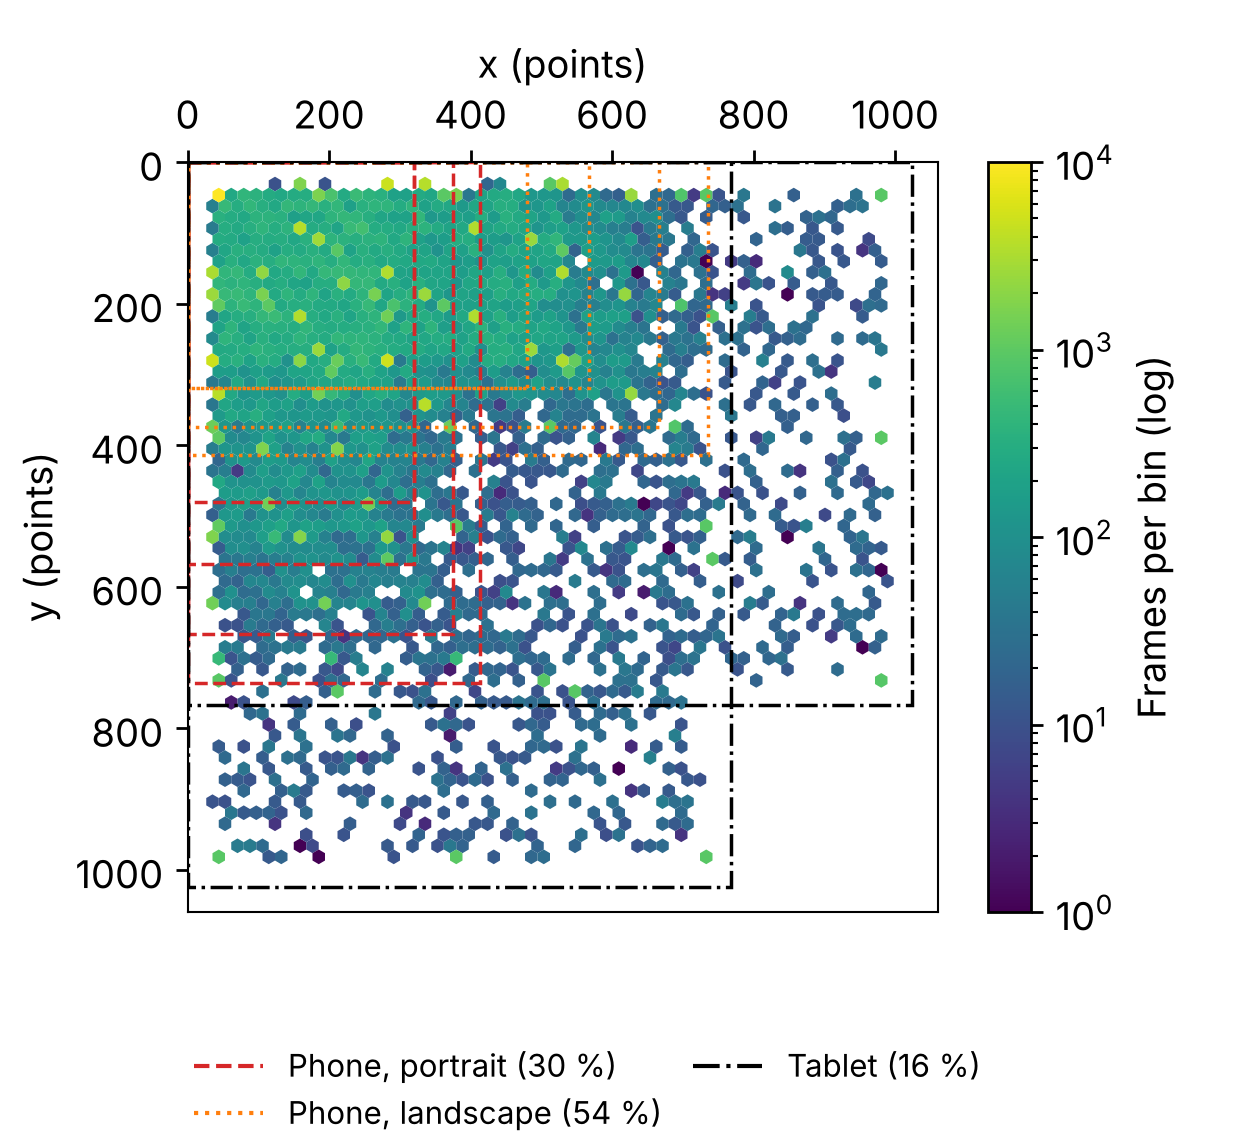
\includegraphics[width=\textwidth]{raw_targets.png}
    \caption{Raw targets in screen points}
    \label{fig:raw_targets}
  \end{subfigure}
  \hfill
  \begin{subfigure}[t]{0.49\textwidth}
    \centering
    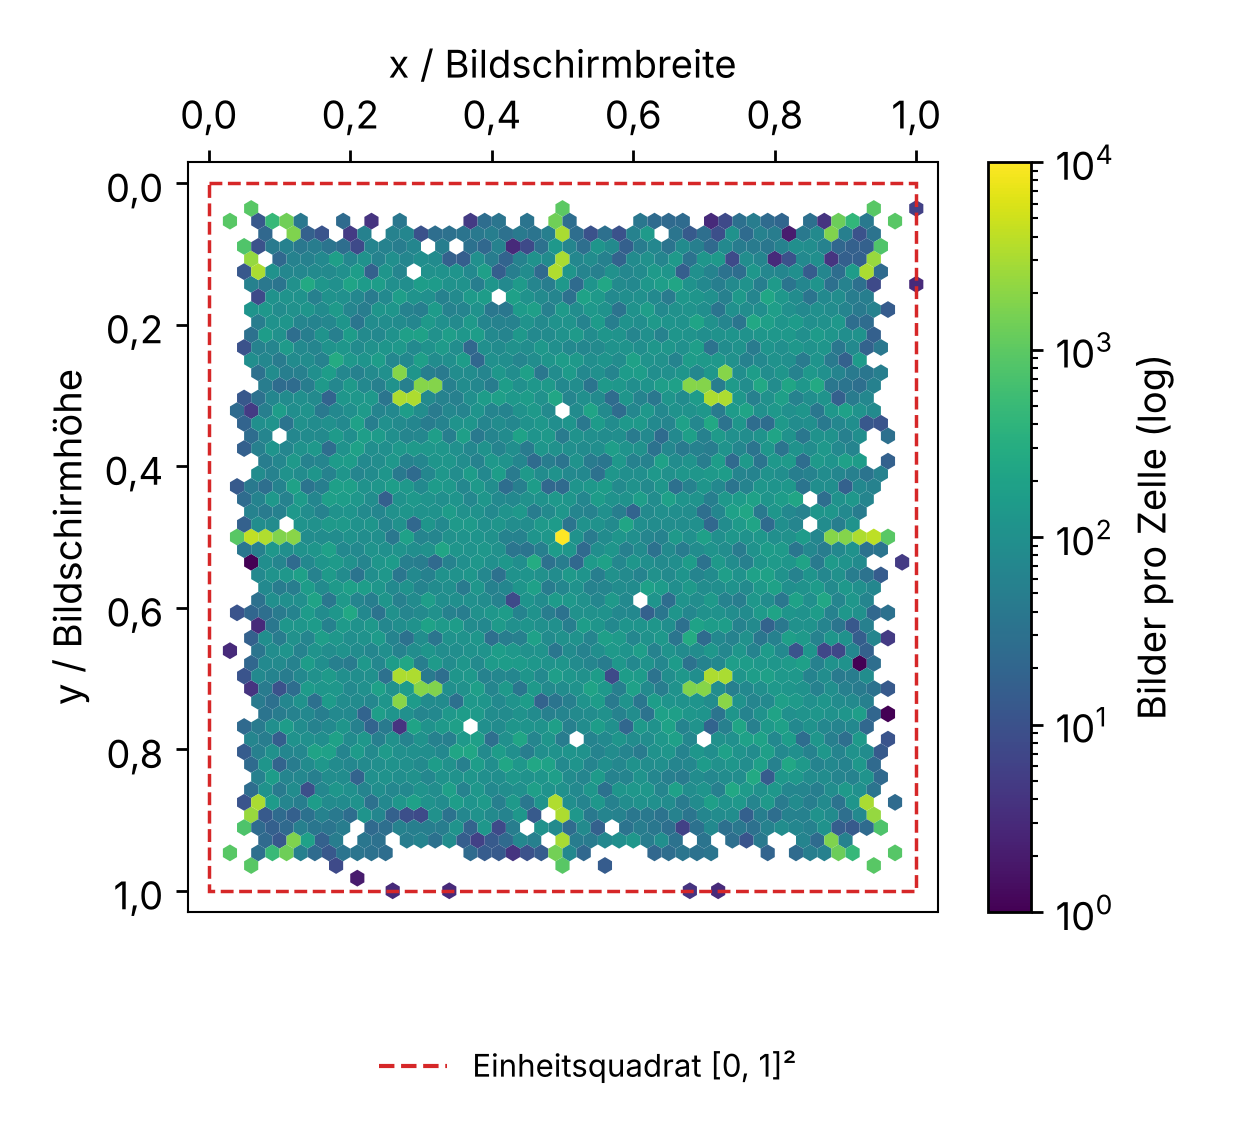
\includegraphics[width=\textwidth]{normalized_targets.png}
    \caption{Normalized targets in the unit square}
    \label{fig:normalized_targets}
  \end{subfigure}
  \caption[GazeCapture gaze targets before and after normalization]{Distribution of the GazeCapture gaze targets before and after
           normalization (density of all frames, logarithmic colour scale).
           Left: dashed, the outlines of the screen formats. Right: dashed, the
           unit square; the bright cells are calibration points that are shown
           at the same relative places on all devices.}
  \label{fig:normalization}
\end{figure}

% ------------------------------------------------------------------------------
\subsection{Baselines}
\label{sec:baselines}

I use two simple reference estimators. The \emph{constant baseline} predicts the
mean of the training targets for every test image. The \emph{random baseline}
draws predictions uniformly from $[0,1]^2$. A model is only useful if it is
clearly better than the constant baseline. An untrained model is not at the
random baseline, but at the constant baseline: its last layer outputs values
close to $0$, the sigmoid turns them into $0.5$, and the model predicts roughly
the screen centre for all images. A learning effect therefore only shows when
the error is \emph{below} the constant baseline of the same test data.

\begin{table}[htbp]
  \centering
  \caption[Baseline errors $\Ediag$ in \si{\percent}]{Baseline errors $\Ediag$ in \si{\percent}. Top: whole dataset
           (bootstrap with 30 samples of 2000 frames each, mean
           and \SI{98}{\percent} CI). Bottom: the same random training/test
           subsets (seed 0) as used for model training (no CI, one fixed
           subset).}
  \label{tab:baselines}
  \small
  \begin{tabular}{lcc}
    \toprule
    Data & Constant baseline & Random baseline \\
    \midrule
    Whole dataset (\num{347085} frames) & 27.28 \,[27.15, 27.40] & 39.82 \,[39.60, 40.04] \\
    \midrule
    \code{norm\_subject}, \num{1000}/\num{200}   & 28.46 & 40.36 \\
    \code{norm\_subject}, \num{10000}/\num{2000} & 27.62 & 39.96 \\
    \code{norm\_random}, \num{1000}/\num{200}    & 27.66 & 39.83 \\
    \bottomrule
  \end{tabular}
\end{table}

The lower part of \cref{tab:baselines} is the correct reference for all model
results in \cref{sec:training}, because it was computed on the same data.

% ==============================================================================
\section{Training Settings}
\label{sec:training}
% ==============================================================================

All results in this section come from one common series of experiments
(corrected metric, random subsets with a fixed seed, early stopping on
validation, five repeats per setting). The constant baseline of the default
setting on the same data is \SI{28.46}{\percent}.

% ------------------------------------------------------------------------------
\subsection{Batch Size}
\label{sec:batch}

\begin{table}[htbp]
  \centering
  \caption[Batch size]{Batch size. Mean test error over five runs with
           \SI{98}{\percent} CI and mean duration of a whole training run (head
           on stored features, see \cref{sec:protocol}).}
  \label{tab:batch_size}
  \small
  \begin{tabular}{ccccc}
    \toprule
    Batch size & Mean test error (\%) & \SI{98}{\percent} CI (\%) & $p$ vs.\ $\dagger$ & Run time (min) \\
    \midrule
    32\sel{}     & 28.39 & [28.21, 28.58] & ---  & 0.019 \\
    64           & 28.35 & [28.29, 28.41] & 0.69 & 0.012 \\
    128          & 28.38 & [28.30, 28.47] & 0.84 & 0.009 \\
    \bottomrule
  \end{tabular}
\end{table}

The three batch sizes give the same test error (\cref{tab:batch_size}): the
means differ by at most \num{0.05} percentage points, the confidence intervals
overlap, and the rank test finds no difference ($p\ge0.69$). A run takes less
than one second, because only the small head is trained on stored features. The
time differences therefore do not matter.

I keep batch size 32 as the default. The experiment shows no disadvantage, and
two practical reasons speak for a small batch size in personalization: (i) a
personal session has only a few hundred training images, and small batches
give more updates per epoch; (ii) the noise of small batches is commonly
thought to have a slight regularizing effect. The data of this experiment,
however, do not \emph{prove} an advantage of 32 over 64 or 128.

% ------------------------------------------------------------------------------
\subsection{Learning Rate}
\label{sec:lr}

\begin{table}[htbp]
  \centering
  \caption[Learning rate]{Learning rate. Mean test error over five runs with
           \SI{98}{\percent} CI and mean duration of a whole training run.}
  \label{tab:learning_rate}
  \small
  \begin{tabular}{ccccc}
    \toprule
    Learning rate & Mean test error (\%) & \SI{98}{\percent} CI (\%) & $p$ vs.\ $\dagger$ & Run time (min) \\
    \midrule
    $10^{-3}$          & 28.43 & [28.33, 28.54] & 0.15  & 0.018 \\
    $10^{-4}$\sel{}    & 28.37 & [28.32, 28.42] & ---   & 0.020 \\
    $10^{-5}$          & 28.33 & [28.28, 28.38] & 0.056 & 0.022 \\
    $10^{-6}$          & 28.37 & [28.21, 28.52] & 0.42  & 0.055 \\
    \bottomrule
  \end{tabular}
\end{table}

\begin{figure}[htbp]
  \centering
  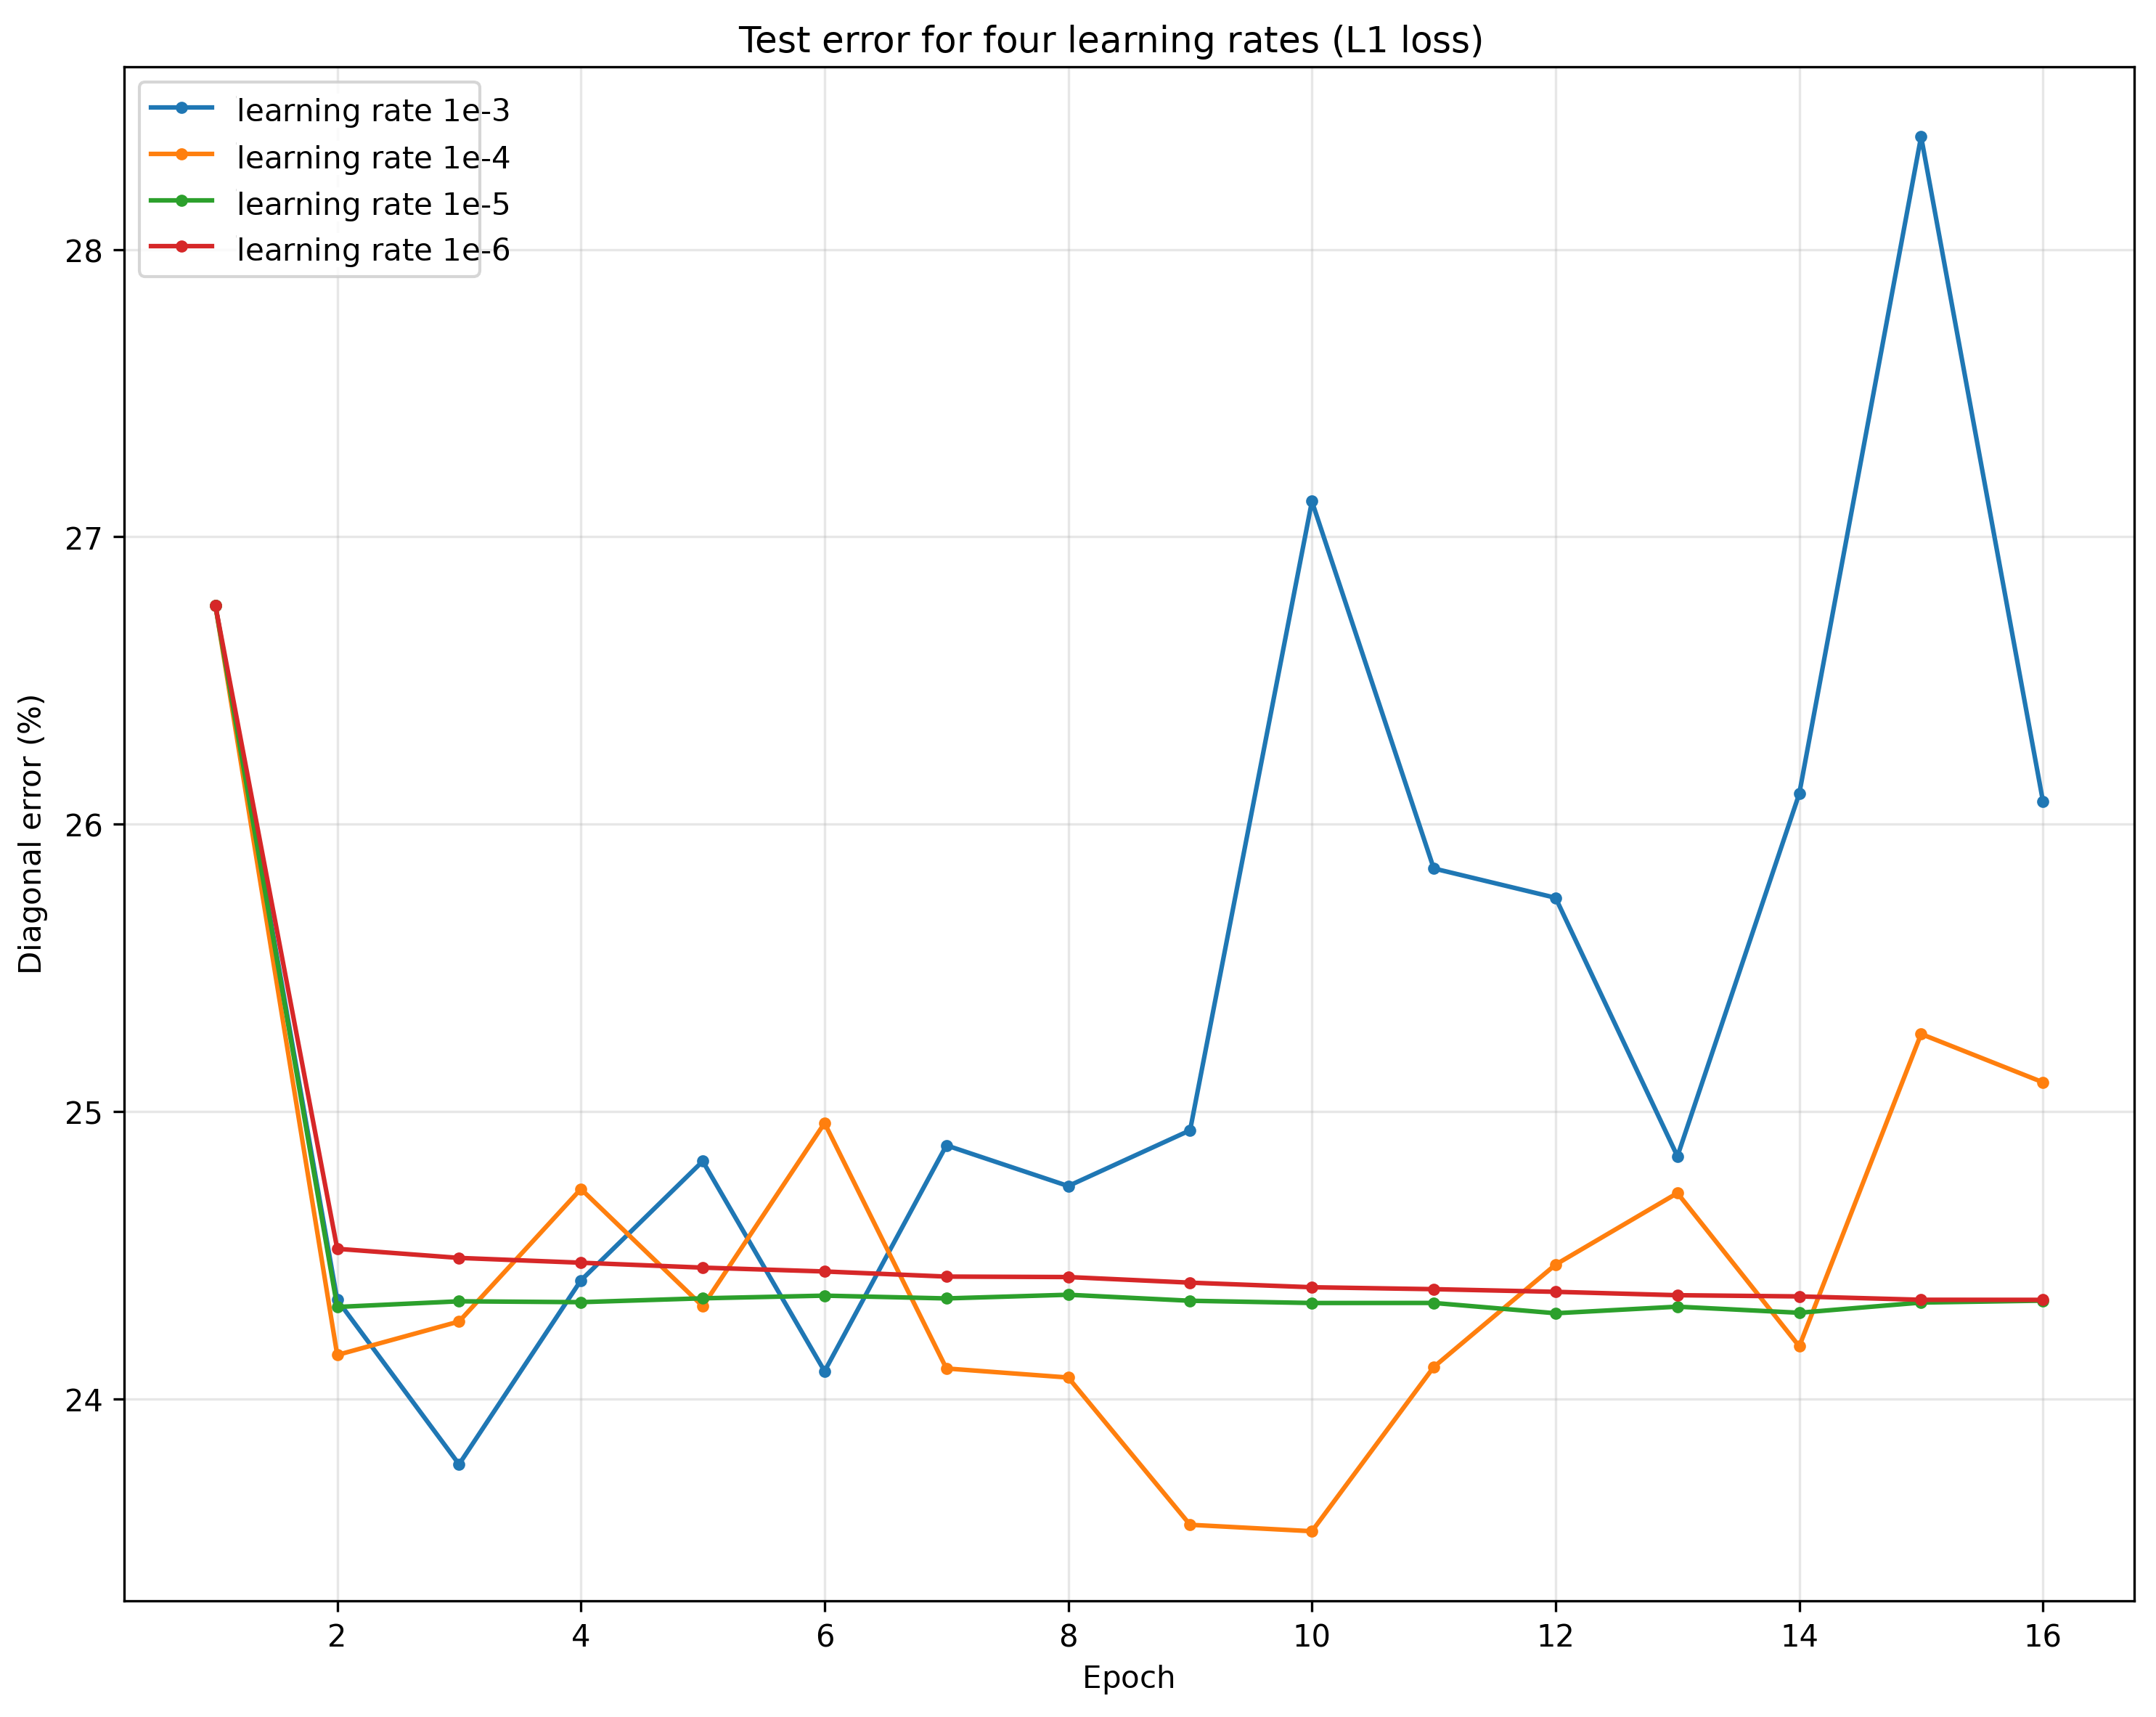
\includegraphics[width=0.78\textwidth]{Test-Error_diff_learning-rate.png}
  \caption[Test error of single runs with four learning rates]{Test error of single training runs with four learning rates
           from an older notebook run (\code{norm\_random},
           \num{1000}/\num{200}, older data selection, 15 epochs without
           early stopping). The first point (epoch~1 on the axis) is the
           untrained model. The values are not directly comparable with
           \cref{tab:learning_rate}.}
  \label{fig:lr_curves}
\end{figure}

The learning rate also shows no significant difference
(\cref{tab:learning_rate}): all means lie between \SI{28.33}{\percent} and
\SI{28.43}{\percent}, the intervals overlap, and no rank test is significant
($p\ge0.056$). So the final error alone cannot justify the choice. The
deciding factor is the first test, i.e.\ the \emph{learning behaviour} in
\cref{fig:lr_curves}:
\begin{itemize}[nosep]
  \item $\bm{\eta = 10^{-3}}$: The steps are too large. After a fast drop, the
        test error jumps up and down and rises again (peaks at about
        \SI{27.1}{\percent} and \SI{28.4}{\percent}). The run does not find a
        stable minimum.
  \item $\bm{\eta = 10^{-4}}$: clearly reaches the lowest test error of all
        curves (about \SI{23.6}{\percent} around epoch~10, i.e.\ about
        0.7~percentage points below $10^{-5}$ and $10^{-6}$). The curve still
        moves, but much less than for $10^{-3}$. Early stopping can keep this
        best state.
  \item $\bm{\eta = 10^{-5}}$ \textbf{and} $\bm{10^{-6}}$: The curves are very
        smooth and fall steadily, but stop at about \SI{24.3}{\percent}. The
        steps are too small to get further in the available time. The result is
        stable, but not the best.
\end{itemize}
The run time also speaks for $10^{-4}$ (\cref{tab:learning_rate}): with
\SI{0.020}{\min} (about \SI{1.2}{\second}) it is among the fastest values.
Only $10^{-3}$ is marginally faster, but unstable; $10^{-6}$ needs almost three
times as long (\SI{0.055}{\min}), because training with very small steps stops
later. I therefore choose $\eta = 10^{-4}$: lowest error in the first test, a
calm learning behaviour and a short run time. The repetition with five runs also
shows that the head on stored features is robust to the learning rate: none of
the other values is significantly better.

% ------------------------------------------------------------------------------
\subsection{Trainable Layers}
\label{sec:layers}

I compare three depths of fine-tuning (\cref{tab:params}): only the regression
head (FC only), the head plus the last residual stage (layer~4), and the
whole network.

\begin{table}[htbp]
  \centering
  \caption{Trainable parameters of the three variants (ResNet-18 with
           regression head, \num{11603650} parameters in total).}
  \label{tab:params}
  \small
  \begin{tabular}{lrrr}
    \toprule
    & FC only & FC + layer 4 & Full ResNet \\
    \midrule
    Trainable parameters           & \num{427138} & \num{8820866} & \num{11603650} \\
    Share of all parameters        & \SI{3.68}{\percent} & \SI{76.02}{\percent} & \SI{100.00}{\percent} \\
    Backbone features can be stored & yes & no & no \\
    \bottomrule
  \end{tabular}
\end{table}

\begin{table}[htbp]
  \centering
  \caption[Trainable layers]{Trainable layers. Mean test error over five runs with
           \SI{98}{\percent} CI and mean duration of a whole training run. For
           \enquote{FC only}, no image passes through the backbone (stored
           features).}
  \label{tab:layers}
  \small
  \begin{tabular}{lcccc}
    \toprule
    Trainable layers & Mean test error (\%) & \SI{98}{\percent} CI (\%) & $p$ vs.\ $\dagger$ & Run time (min) \\
    \midrule
    FC only\sel{}          & 28.36 & [28.23, 28.49] & ---  & 0.015 \\
    FC + layer 4           & 29.07 & [26.58, 31.55] & 0.22 & 9.160 \\
    Full ResNet            & 29.39 & [26.99, 31.78] & 0.31 & 15.366 \\
    \bottomrule
  \end{tabular}
\end{table}

\enquote{FC only} has the lowest mean error and by far the narrowest interval
(\cref{tab:layers}). More trainable layers do not help. They even make the
result \emph{less reliable}: one run with FC + layer~4 (\SI{31.72}{\percent})
and two runs with the full ResNet (\SI{30.70}{\percent} and
\SI{31.18}{\percent}) end clearly above the constant baseline
(\SI{28.46}{\percent}). All runs with \enquote{FC only} stay between
\SI{28.28}{\percent} and \SI{28.47}{\percent}. With only five runs, the
differences are not significant ($p=0.22$ and $0.31$), so the value for
\enquote{FC only} is not bold. Training time grows strongly with the number of
parameters: \SI{9.2}{\minute} per run for FC + layer~4 and \SI{15.4}{\minute}
for the whole network.

I choose \enquote{FC only} for three reasons:
\begin{enumerate}[nosep]
  \item \textbf{Not worse, but more stable:} more layers do not lower the error
        here; they only increase the spread between runs.
  \item \textbf{Robust with little data:} a personal session has only a few
        hundred images. Training millions of backbone parameters with so few
        examples risks overfitting and distorts the pretrained features.
        \citet{kumar2022finetuning} show that full fine-tuning can damage
        pretrained features and generalize worse than head-only training.
  \item \textbf{Effort:} only \SI{3.68}{\percent} of the parameters are
        trained, and the backbone features are computed only once. This makes
        personalization fast and memory-friendly.
\end{enumerate}

% ------------------------------------------------------------------------------
\subsection{Output Activation}
\label{sec:activation}

The output activation comes after the last linear layer, which outputs $(x,y)$.
Sigmoid maps to $(0,1)$, which is exactly the range of the normalized
coordinates. The Gaussian activation $g(z)=\exp(-z^2/2\sigma^2)$ with $\sigma=1$
maps to $(0,1]$, but it is not monotonic. ReLU only removes negative values, and
\enquote{None} leaves the output unchanged.

\begin{table}[htbp]
  \centering
  \caption[Output activation]{Output activation. Mean test error over five runs with
           \SI{98}{\percent} CI and mean duration of a whole training run.}
  \label{tab:activation}
  \small
  \begin{tabular}{lcccc}
    \toprule
    Activation & Mean test error (\%) & \SI{98}{\percent} CI (\%) & $p$ vs.\ $\dagger$ & Run time (min) \\
    \midrule
    Sigmoid\sel{}    & \textbf{28.36} & [28.29, 28.43] & ---   & 0.022 \\
    Gaussian         & 31.29 & [28.44, 34.14] & 0.008 & 0.019 \\
    ReLU             & 32.90 & [19.69, 46.10] & 0.008 & 0.028 \\
    None             & 29.39 & [28.42, 30.36] & 0.008 & 0.032 \\
    \bottomrule
  \end{tabular}
\end{table}

Sigmoid is the only clear winner of the hyperparameter study
(\cref{tab:activation}): lowest error, narrowest interval, and \emph{every}
sigmoid run is better than \emph{every} run of the three other activations
($p=0.008$ in all three comparisons). The value is therefore bold. The other
activations are also less stable: one ReLU run ends at \SI{46.98}{\percent},
which is worse than random guessing. A possible reason: ReLU can output zero for
all inputs (\enquote{dead} output), and the gradient does not recover from
this. Without a bounding activation (None, ReLU), the network can also predict
points outside the screen. I choose sigmoid because it keeps the output on the
screen and gives the lowest and most stable error.

% ------------------------------------------------------------------------------
\subsection{Amount of Data}
\label{sec:size}

\begin{table}[htbp]
  \centering
  \caption[Amount of data (training/test)]{Amount of data (training/test). Mean test error over five runs
           with \SI{98}{\percent} CI, mean duration of a whole training run and
           constant baseline of the respective test data.}
  \label{tab:dataset_size}
  \small
  \setlength{\tabcolsep}{3.5pt}
  \begin{tabular}{lccccc}
    \toprule
    Training / test & Mean test error (\%) & \SI{98}{\percent} CI (\%) & $p$ vs.\ $\dagger$ & Run time (min) & Const.\ baseline (\%) \\
    \midrule
    \num{10000} / \num{2000}      & 27.64 & [27.55, 27.73] & 0.008 & 0.167 & 27.62 \\
    \num{1000} / \num{200}\sel{}  & 28.39 & [28.33, 28.44] & ---   & 0.018 & 28.46 \\
    \bottomrule
  \end{tabular}
\end{table}

The larger amount of data has a lower mean error (\cref{tab:dataset_size}). But
the two variants are evaluated on \emph{different} test data, and each mean is
practically equal to the constant baseline of its own test data
(\SI{27.64}{\percent} vs.\ \SI{27.62}{\percent} and \SI{28.39}{\percent} vs.\
\SI{28.46}{\percent}). The difference of \num{0.75} percentage points therefore
comes from the different test data and not from more training data -- even
though the rank test is significant ($p=0.008$). I keep the small variant
(\num{1000}/\num{200}) because it is about ten times faster and has about as
much data as a personalization session.

% ------------------------------------------------------------------------------
\subsection{Type of Split}
\label{sec:split}

\begin{table}[htbp]
  \centering
  \caption[Type of split]{Type of split. Mean test error over five runs with
           \SI{98}{\percent} CI and constant baseline of the respective test
           data.}
  \label{tab:split}
  \small
  \begin{tabular}{lcccc}
    \toprule
    Split & Mean test error (\%) & \SI{98}{\percent} CI (\%) & $p$ vs.\ $\dagger$ & Constant baseline (\%) \\
    \midrule
    \code{norm\_random}           & 27.72 & [27.64, 27.80] & 0.008 & 27.66 \\
    \code{norm\_subject}\sel{}    & 28.39 & [28.26, 28.53] & ---   & 28.46 \\
    \bottomrule
  \end{tabular}
\end{table}

The random split gives the lower error (\cref{tab:split}). Here, too, most of
the difference comes from the test data: the constant baseline is already
\num{0.80} percentage points lower on \code{norm\_random}, and both models lie
at most \num{0.07} percentage points away from their baseline. In addition, the
random split allows the same persons in training and test. This makes the task
easier and the result too optimistic. I therefore use \code{norm\_subject} as
the default. Only this split measures the performance on unknown persons, that
is, the situation before personalization.

% ==============================================================================
\section{Spatial Error Analysis and Loss Functions}
\label{sec:spatial}
% ==============================================================================

The mean error from \cref{sec:training} does not show \emph{where} on the screen
the errors occur. This section first studies the spatial distribution of the
error (\cref{sec:partition,sec:heatmaps}). The result led to the idea of
weighting the loss by position (\cref{sec:losses}). \Cref{sec:loss_results}
evaluates this idea.

\subsection{Screen Partition}
\label{sec:partition}

I describe the normalized screen $[0,1]^2$ with a $3\times3$ grid of three
regions:
\begin{align*}
  \text{Centre:}  &\quad (0.50, 0.50),\\
  \text{Edges:}   &\quad (0.10, 0.50),\ (0.50, 0.10),\ (0.90, 0.50),\ (0.50, 0.90),\\
  \text{Corners:} &\quad (0.10, 0.10),\ (0.10, 0.90),\ (0.90, 0.10),\ (0.90, 0.90).
\end{align*}
A test example with target $\bm p$ belongs to grid point $\bm g$ if
$\lVert\bm p-\bm g\rVert_2 \le r$ with $r = 0.15$. The error of a grid point is
the mean Euclidean error $\lVert\hat{\bm p}-\bm p\rVert_2$ of its examples (in
normalized units, that is, as a share of the screen side; the diagonal is
$\sqrt2 \approx 1.41$). The error of a region is the mean over all examples of
its grid points. These definitions apply to all figures and tables in this
section.

\subsection{Error Heat Maps}
\label{sec:heatmaps}

\Cref{fig:heatmaps} uses the 200 test predictions of the default model
(\code{norm\_subject}, L1 loss).
For a position $\bm c$ (centre, edge or corner), I compute the mean error
$\bar e(\bm c)$ of all examples within radius $r$ and draw it as a Gaussian
spot:
\begin{equation}
  H(x,y) = \bar e(\bm c)\,
  \exp\!\left(-\frac{\lVert (x,y)-\bm c\rVert_2^2}{2\sigma^2}\right),
  \qquad \sigma = 0.20 .
\end{equation}
So the colour shows the \emph{size} of the local error, and the position of the
bright spot shows \emph{where} it was measured. All three panels use the same
colour scale (from 0 to the largest value), so the colours can be compared
directly.

\begin{figure}[htbp]
  \centering
  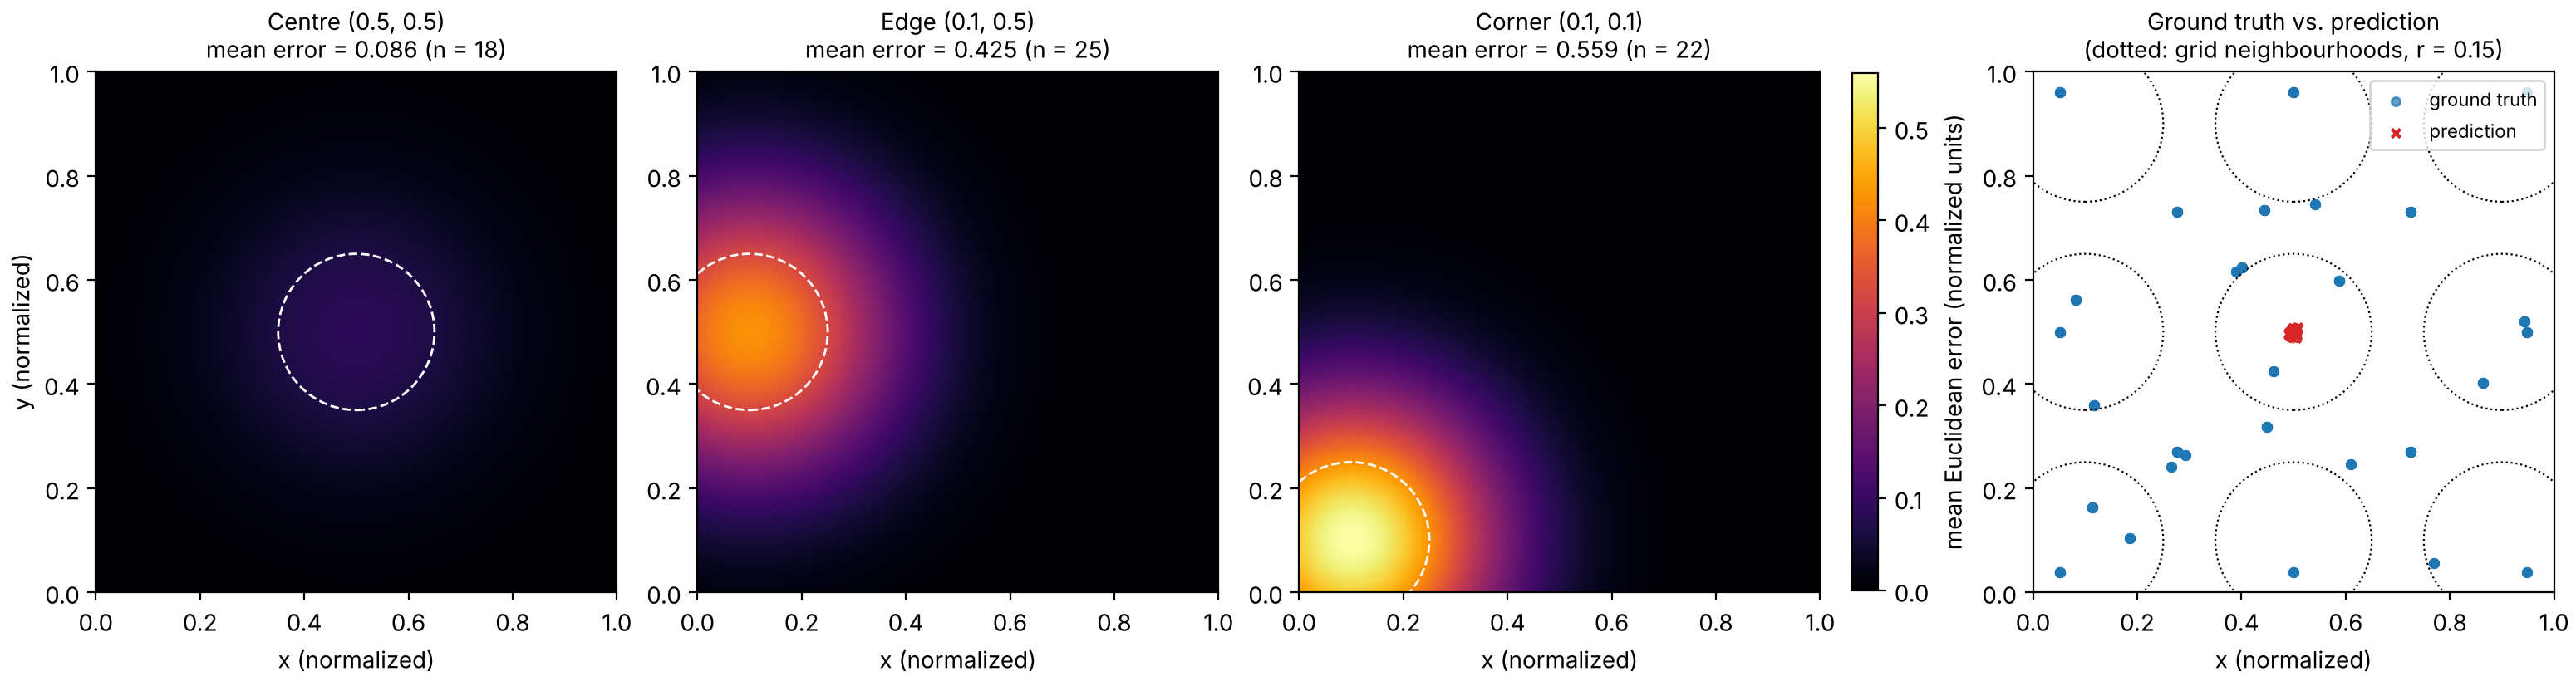
\includegraphics[width=\textwidth]{fig4_spatial_heatmaps.png}
  \caption[Spatial error of the default model]{Spatial error of the default model (L1 loss, \code{norm\_subject},
           200 test examples). Panels 1--3: error heat maps ($r=0.15$,
           $\sigma=0.20$, common colour scale) at the centre $(0.5, 0.5)$, the
           left edge $(0.1, 0.5)$ and the bottom left corner $(0.1, 0.1)$. The
           error grows from the centre (0.086) over the edge (0.425) to the
           corner (0.559). Panel 4: targets (blue) and predictions (red); all
           predictions lie close to the screen centre.}
  \label{fig:heatmaps}
\end{figure}

The error grows from the inside to the outside: it is $0.086$ in the centre
($n=18$), $0.432$ at the edges ($n=62$) and $0.586$ in the corners ($n=42$). The
edge errors are about five times and the corner errors about seven times as
large as in the centre.

The fourth panel explains the reason. All predictions lie in a very small area
around $(0.5, 0.5)$. Their standard deviation is only about $0.004$ in both
coordinates, while that of the targets is about $0.28$. So the model predicts
almost the same point for every image. Its error is simply the distance of the
target from the screen centre. An estimator that always outputs the centre gives
practically the same values (centre $0.085$, edges $0.432$, corners $0.587$; in
total $\Ediag=\SI{28.45}{\percent}$ compared with \SI{28.47}{\percent} for the
model).

\subsection{Loss Functions}
\label{sec:losses}

Because of the large errors at the edges and corners, the idea came up to give
these areas more weight in the loss. Let $\hat{\bm p}_i=(\hat x_i,\hat y_i)$ be
the prediction and $\bm p_i=(x_i,y_i)$ the target of example $i$ in a batch of
size $N$.

\paragraph{L1 loss.}
\begin{equation}
  \mathcal{L}_{1} = \frac{1}{2N}\sum_{i=1}^{N}\bigl(|\hat x_i-x_i| + |\hat y_i-y_i|\bigr).
\end{equation}
The gradient always has the same size, no matter how large the error is. The
loss is therefore robust against outliers (for example wrong labels during
target changes), but it treats all screen positions the same.

\paragraph{Smooth L1 loss ($\beta=1$).}
For a residual $u$:
\begin{equation}
  \ell_\beta(u) =
  \begin{cases}
    \dfrac{u^2}{2\beta}, & |u| < \beta,\\[1.2ex]
    |u| - \dfrac{\beta}{2}, & \text{otherwise.}
  \end{cases}
\end{equation}
It is quadratic for small and linear for large residuals. Because all residuals
here are smaller than $\beta=1$, it behaves like a scaled squared error: for
small errors the gradient becomes small.

\paragraph{Sensitive L1 loss (weighted by position).}
Each example is weighted with its $L_1$ distance to the screen centre:
\begin{equation}
  d_i = |x_i-0.5| + |y_i-0.5| \in [0,1],\qquad
  w_i = 1 + d_i \in [1,2],
\end{equation}
\begin{equation}
  \mathcal{L}_{\mathrm{sens}} = \frac{1}{N}\sum_{i=1}^{N}
  w_i\cdot\frac{|\hat x_i-x_i| + |\hat y_i-y_i|}{2}.
\end{equation}
An example in a corner counts twice as much as one in the centre, an example at
an edge about $1.4$ times as much. The gradient for outer targets becomes
larger, and this should pull the predictions away from the centre.

The \enquote{improved sensitive loss} in \cref{tab:loss_aux} was another
variant from an early trial. Its exact formula is no longer documented; it is
listed only for completeness.

\subsection{Results: Comparison of the Loss Functions}
\label{sec:loss_results}

\Cref{tab:loss} shows the global comparison with five runs together with the
errors in the screen regions from \cref{sec:partition}.

\begin{table}[htbp]
  \centering
  \caption[Comparison of L1 and sensitive L1 loss]{Comparison of L1 and sensitive L1 loss. Left: mean test error
           $\Ediag$ over five runs (\SI{98}{\percent} CI) and
           mean run time. Right: mean Euclidean error per screen region
           (normalized units; one run each, 200 test examples, $r=0.15$; $n$ =
           number of examples). Last row: estimator that always outputs the
           centre, on the same 200 test examples.}
  \label{tab:loss}
  \small
  \setlength{\tabcolsep}{4.5pt}
  \begin{tabular}{lccc@{\hspace{1.2em}}ccc}
    \toprule
    & \multicolumn{3}{c}{Global (5 runs)} & \multicolumn{3}{c}{Spatial error (1 run)} \\
    \cmidrule(lr){2-4}\cmidrule(lr){5-7}
    Loss & $\Ediag$ (\%) & \SI{98}{\percent} CI (\%) & Run time (min)
         & Centre & Edges & Corners \\
         &               &                           &
         & ($n=18$) & ($n=62$) & ($n=42$) \\
    \midrule
    L1 (standard)\sel{}    & \textbf{28.32} & [28.23, 28.42] & 0.011 & 0.086 & 0.432 & 0.586 \\
    Sensitive L1           & 28.48 & [28.19, 28.78] & 0.021 & 0.090 & 0.431 & 0.585 \\
    \midrule
    Constant centre        & 28.45\textsuperscript{a} & --- & --- & 0.085 & 0.432 & 0.587 \\
    \bottomrule
  \end{tabular}\\[1mm]
  \parbox{0.95\linewidth}{\footnotesize \textsuperscript{a}\,On the same 200 test
  examples as the spatial analysis.}
\end{table}

\begin{table}[htbp]
  \centering
  \caption[Additional experiment: spatial error of four loss functions]{Additional experiment: spatial error of four loss functions after
           15 epochs on training data with 52 corner examples (two runs, A and
           B, values as logged). The numbers come from a notebook for trying
           things out. The computation of the region values is not in the
           current code; they are therefore not directly comparable with
           \cref{tab:loss}.}
  \label{tab:loss_aux}
  \small
  \setlength{\tabcolsep}{5pt}
  \begin{tabular}{l cc cc cc cc}
    \toprule
    & \multicolumn{2}{c}{Overall (\%)} & \multicolumn{2}{c}{Centre (\%)}
    & \multicolumn{2}{c}{Edges (\%)} & \multicolumn{2}{c}{Corners (\%)} \\
    \cmidrule(lr){2-3}\cmidrule(lr){4-5}\cmidrule(lr){6-7}\cmidrule(lr){8-9}
    Loss & A & B & A & B & A & B & A & B \\
    \midrule
    L1                                & 24.54 & 24.63 & 17.01 & 16.74 & 28.28 & 28.98 & 34.93 & 35.07 \\
    Smooth L1                         & 23.94 & 24.91 & 15.40 & 16.41 & 29.78 & 30.59 & 34.13 & 35.17 \\
    Sensitive L1                      & 25.57 & 25.55 & 19.11 & 18.61 & 29.87 & 29.93 & 33.41 & 34.20 \\
    Improved sensitive L1             & 25.53 & 27.75 & 19.20 & 21.86 & 29.17 & 35.03 & 33.77 & 31.58 \\
    \bottomrule
  \end{tabular}
\end{table}

\paragraph{Observations.}
\begin{itemize}[nosep]
  \item Globally, L1 is slightly but significantly better than the sensitive
        loss: \SI{28.32}{\percent} compared with \SI{28.48}{\percent}
        (Mann-Whitney $p=0.032$, \cref{tab:loss}); the L1 value is therefore
        bold. The sensitive loss also varies more between runs. Both values
        are close to the constant baseline (\SI{28.46}{\percent}).
  \item Spatially, the weighting changes the region errors by less than
        $0.005$ normalized units. Edge and corner errors stay about five to
        seven times as large as in the centre.
  \item Both models have the same spatial pattern as an estimator that always
        outputs the centre. The weighting does increase the gradient for outer
        examples, but this is not enough for the model to leave the centre.
  \item In the additional experiment (\cref{tab:loss_aux}), the sensitive
        variants lower the corner error a little (sensitive L1 by
        \num{0.9}--\num{1.5}, the improved variant by \num{1.2}--\num{3.5}
        percentage points). But they raise the centre error by
        \num{1.9}--\num{5.1} percentage points and the overall error in all
        runs. The two runs differ a lot; these trends are therefore not
        reliable.
\end{itemize}

\paragraph{Conclusion.}
The spatial analysis shows \emph{what} the problem is: the errors lie mainly at
the edges and in the corners. The weighted loss was meant to reduce these
errors. It did not improve the corners and was globally even slightly but
significantly worse than L1 ($p=0.032$). In the additional experiment it raised
the error in the centre. I therefore keep the normal L1 loss: it has the lower
error, is simpler, has no extra parameter, and its constant gradient makes it
robust against wrong labels in the own recordings. The analysis also shows
\emph{why} the weighting could not help: the large outer errors are not caused
by a wrong weighting, but by the model hardly leaving the screen centre
(\cref{sec:discussion}).

% ==============================================================================
\section{Personalization Sessions}
\label{sec:sessions}
% ==============================================================================

\subsection{Setup}
\label{sec:sessions_setup}

In each personal session, the head of a GazeCapture base model is trained
further on the frames of one own recording (FC only, sigmoid, L1,
$\eta=10^{-4}$, weight decay $10^{-5}$, batch size 32, AdamW). Unless stated
otherwise, each session is split randomly into \SI{70}{\percent} training,
\SI{15}{\percent} validation and \SI{15}{\percent} test (seed 42). Early
stopping (patience 3) uses the validation error. I report the test error at the
epoch with the lowest validation error. If the best epoch is 0, personalization
did not improve the validation error. The reported test error is then that of
the unchanged base model.

All results from here on use the corrected metric (\cref{eq:ediag}) and fixed
random seeds. The backbone, including its
BatchNorm statistics, is completely frozen.

\paragraph{Stored features.} Because the backbone is frozen, it gives the same 512
features for an image in every epoch. I therefore compute these features only
once per session and base model (without augmentation) and store them. After
that, only the head is trained. This does not change the result, but a run
takes only seconds on a CPU. No image augmentation is used during
personalization.

\paragraph{Base models (E0).} The two base models are trained with the setting
from \cref{sec:training} (FC only, sigmoid, L1, $\eta=10^{-4}$, batch size 32,
\num{1000}/\num{200} random frames, seed~0, early stopping on validation) on
\code{norm\_subject} and \code{norm\_random}. Of five seeds, I keep the run with
the lowest \emph{validation} error. For \code{norm\_subject} this is seed~0 (validation
\SI{27.37}{\percent}, test \SI{28.70}{\percent}; constant baseline of the same
test data \SI{28.46}{\percent}), for \code{norm\_random} seed~3 (validation
\SI{26.74}{\percent}, test \SI{27.81}{\percent}; constant baseline
\SI{27.66}{\percent}). The five seeds differ by less than \num{0.4} percentage
points, so the choice of seed is not critical. As described in
\cref{sec:discussion}, both base models are at the level of the constant
baseline.

Of 27 recorded sessions, I use 18: Gen~1 (01--04), Gen~2 (05--09) and Gen~4
(19--27). I discarded Gen~3 (10--18) because the model could not learn anything
from it. \Cref{tab:session_conditions} shows the recording conditions.

\begin{table}[htbp]
  \centering
  \caption[Recording conditions of the 18 sessions]{Recording conditions of the 18 sessions. Gen~1: target moves
           smoothly, without jumps; Gen~2: target with random jumps; Gen~4:
           5-s segments (\SI{0.5}{\second} WAIT at a new start point,
           \SI{4.5}{\second} MOVE), \SI{90}{\percent} of the start points in the
           corners. The length was only changed in Gen~4 (Gen~1/2: not
           logged). Device~A: sessions 01--03 and 25--27; device~B: 05--09
           and 19--24; session 04: not logged.}
  \label{tab:session_conditions}
  \small
  \begin{tabular}{llll}
    \toprule
    Sessions & Generation & Glasses & Light / background \\
    \midrule
    01, 03, 04 & Gen 1 & with    & 01, 04: bright; 03: dark \\
    02         & Gen 1 & without & bright \\
    05, 07, 08 & Gen 2 & with    & 05: bright; 07: dark; 08: very dark \\
    06, 09     & Gen 2 & without & 06: bright; 09: very dark \\
    \midrule
    \multicolumn{4}{l}{Gen 4 \quad (length / device)} \\
    19, 20 & Gen 4 & with    & calm; 120\,s / 90\,s; B \\
    21, 22 & Gen 4 & without & calm; 120\,s / 90\,s; B \\
    23 / 24 & Gen 4 & with / without & busy; 120\,s; B \\
    25 / 26 & Gen 4 & with / without & busy; 120\,s; A \\
    27     & Gen 4 & with    & busy; 90\,s; A \\
        \midrule
    28 / 29 (person~B) & Gen 4 & without & bright; calm / busy; 120\,s; A / B \\
    \bottomrule
  \end{tabular}
\end{table}

\subsection{Results of All Sessions (E1)}
\label{sec:sessions_results}

\Cref{tab:sessions} shows every session with both base models.

\begin{table}[htbp]
  \centering
  \caption[Personalization of the 18 sessions with two base models]{Personalization of the 18 sessions with two base models
           (original labels, random 70/15/15 split, seed 42). Base: test error
           of the unchanged base model (epoch~0); Val.: best validation error;
           Test: test error at the best validation epoch; Ep.: best epoch; $t$:
           duration of one run in seconds (\cref{sec:session_time}); Const.:
           constant baseline (mean of the training targets, on the same test
           frames). Errors in \si{\percent} (\cref{eq:ediag}). Group rows: mean
           and \SI{98}{\percent} CI over the sessions of the group.}
  \label{tab:sessions}
  \footnotesize
  \setlength{\tabcolsep}{2.6pt}
  \resizebox{\textwidth}{!}{%
  \begin{tabular}{cc ccccc ccccc c}
    \toprule
    & & \multicolumn{5}{c}{Base model \code{norm\_subject}}
      & \multicolumn{5}{c}{Base model \code{norm\_random}} & \\
    \cmidrule(lr){3-7}\cmidrule(lr){8-12}
    Session & Gen. & Base & Val. & Test & Ep. & $t$ (s) & Base & Val. & Test & Ep. & $t$ (s) & Const. \\
    \midrule
    01 & 1 & 29.19 & 14.82 & 15.83 & 22 & 2.3 & 29.49 & 11.70 & 12.97 & 47 & 4.2 & 29.45 \\
    02 & 1 & 28.48 & 10.08 & 10.48 & 30 & 2.2 & 28.42 & 10.04 & 10.43 & 44 & 3.2 & 28.49 \\
    03 & 1 & 29.61 & 15.26 & 17.20 & 33 & 2.5 & 30.13 & 15.41 & 17.35 & 36 & 2.6 & 29.76 \\
    04 & 1 & 29.98 & 16.88 & 17.64 & 17 & 2.1 & 29.38 & 15.23 & 16.16 & 31 & 2.7 & 29.17 \\
    05 & 2 & 32.92 & 25.43 & 17.64 & 26 & 1.1 & 32.49 & 31.93 & 32.77 & 2 & 0.2 & 32.72 \\
    06 & 2 & 29.29 & 11.31 & 16.67 & 54 & 1.8 & 28.89 & 12.09 & 16.55 & 55 & 2.0 & 27.02 \\
    07 & 2 & 32.18 & 24.84 & 30.99 & 16 & 0.7 & 32.43 & 25.02 & 31.62 & 18 & 0.6 & 32.28 \\
    08 & 2 & 25.82 & 23.65 & 23.30 & 24 & 0.8 & 26.32 & 23.38 & 22.31 & 23 & 0.6 & 27.00 \\
    09 & 2 & 26.83 & 23.55 & 28.64 & 4 & 0.2 & 26.21 & 15.19 & 16.87 & 47 & 1.9 & 28.17 \\
    19 & 4 & 30.42 & 13.38 & 17.76 & 33 & 2.8 & 30.04 & 12.13 & 16.85 & 47 & 4.4 & 30.19 \\
    20 & 4 & 33.14 & 16.06 & 14.64 & 23 & 1.9 & 33.01 & 14.58 & 12.93 & 35 & 2.7 & 33.49 \\
    21 & 4 & 30.18 & 15.03 & 12.51 & 39 & 4.6 & 30.46 & 15.80 & 13.20 & 23 & 2.6 & 29.97 \\
    22 & 4 & 31.17 & 13.54 & 13.02 & 22 & 2.2 & 30.87 & 12.53 & 12.32 & 37 & 3.1 & 30.32 \\
    23 & 4 & 33.15 & 23.48 & 23.65 & 10 & 1.4 & 32.59 & 24.02 & 24.05 & 10 & 2.0 & 32.57 \\
    24 & 4 & 33.09 & 28.77 & 26.97 & 7 & 0.9 & 32.84 & 29.53 & 27.42 & 6 & 1.0 & 33.01 \\
    25 & 4 & 32.19 & 26.98 & 24.61 & 19 & 2.4 & 33.00 & 26.74 & 24.13 & 26 & 2.8 & 31.54 \\
    26 & 4 & 30.60 & 21.93 & 18.61 & 20 & 2.3 & 30.39 & 21.40 & 17.97 & 37 & 4.5 & 29.48 \\
    27 & 4 & 31.98 & 26.05 & 26.06 & 19 & 1.5 & 32.29 & 26.27 & 26.68 & 19 & 1.7 & 31.19 \\
    \midrule
    \multicolumn{2}{l}{Gen 1 (4)} & 29.32 & 14.26 & 15.29 & 25.5 & 2.3 & 29.35 & 13.10 & 14.23 & 39.5 & 3.2 & 29.22 \\
      & & [27.86, 30.77] & [7.62, 20.89] & [7.80, 22.77] & & [1.8, 2.7] & [27.75, 30.96] & [7.07, 19.12] & [7.10, 21.35] & & [1.5, 4.8] & [27.99, 30.45] \\
    \multicolumn{2}{l}{Gen 2 (5)} & 29.41 & 21.76 & 23.45 & 24.8 & 0.9 & 29.27 & 21.52 & 24.02 & 29.0 & 1.0 & 29.44 \\
      & & [24.14, 34.68] & [11.88, 31.63] & [12.74, 34.16] & & [0.0, 1.9]\textsuperscript{a} & [24.06, 34.47] & [8.20, 34.85] & [10.93, 37.12] & & [0.0, 2.5]\textsuperscript{a} & [24.68, 34.20] \\
    \multicolumn{2}{l}{Gen 4 (9)} & 31.77 & 20.58 & 19.76 & 21.3 & 2.2 & 31.72 & 20.33 & 19.51 & 26.7 & 2.8 & 31.31 \\
      & & [30.60, 32.94] & [14.66, 26.50] & [14.26, 25.26] & & [1.2, 3.3] & [30.51, 32.93] & [13.88, 26.79] & [13.59, 25.42] & & [1.7, 3.9] & [29.91, 32.70] \\
    \midrule
    \multicolumn{2}{l}{\textbf{All (18)}} & \textbf{30.57} & \textbf{19.50} & \textbf{19.79} & \textbf{23.2} & \textbf{1.9} & \textbf{30.51} & \textbf{19.05} & \textbf{19.59} & \textbf{30.2} & \textbf{2.4} & \textbf{30.32} \\
      & & [29.27, 31.87] & [15.87, 23.13] & [16.18, 23.40] & & [1.3, 2.5] & [29.21, 31.82] & [14.86, 23.25] & [15.47, 23.71] & & [1.6, 3.2] & [29.12, 31.53] \\
    \bottomrule
  \end{tabular}}\\[1mm]
  \parbox{0.95\linewidth}{\footnotesize \textsuperscript{a}\,The lower limit of
  the $t$ interval is below zero (few sessions, large spread) and was cut at 0.}
\end{table}

\begin{figure}[htbp]
  \centering
  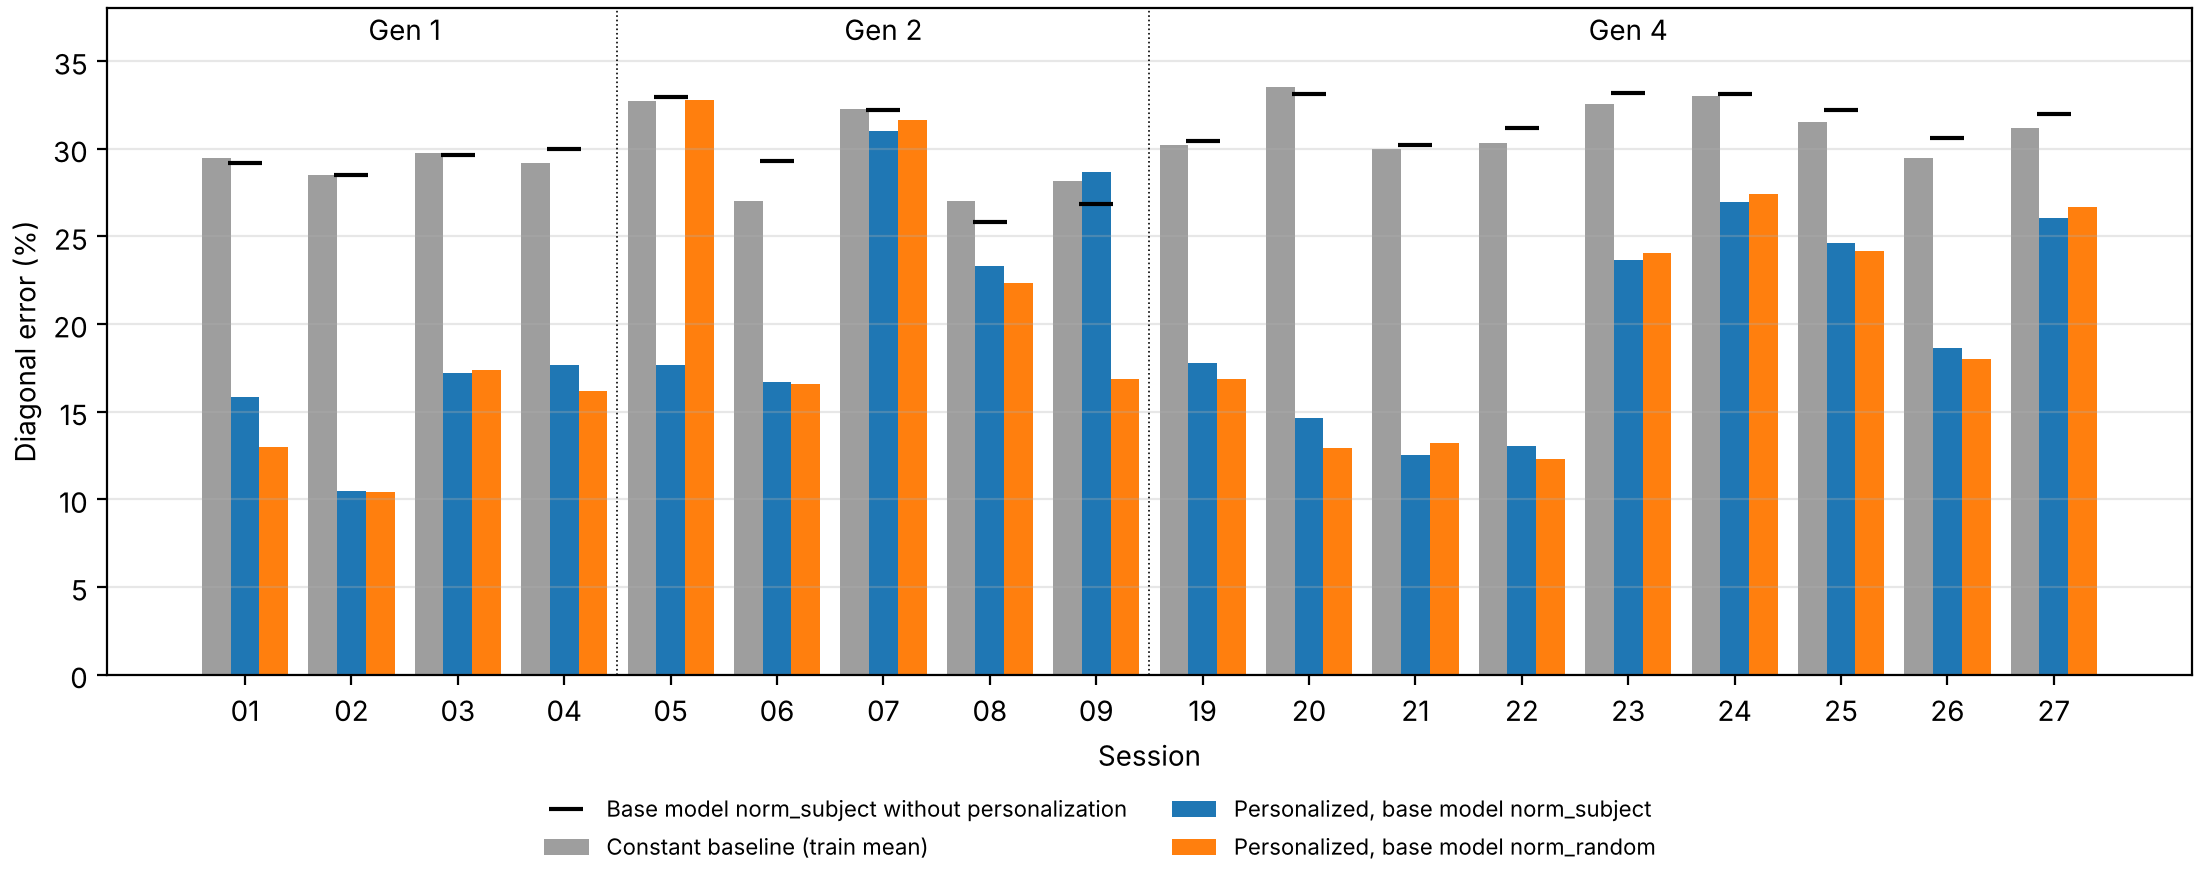
\includegraphics[width=\textwidth]{fig_sessions_baseline.png}
  \caption{Test error of the 18 sessions after personalization with both base
           models, compared with the constant baseline and the unchanged base
           model (\code{norm\_subject}) on the same test frames (data from
           \cref{tab:sessions}).}
  \label{fig:sessions}
\end{figure}

\paragraph{Personalization works.}
Over all 18 sessions, the test error drops from \SI{30.32}{\percent} (constant
baseline) to \SI{19.79}{\percent} with the base model \code{norm\_subject} and
to \SI{19.59}{\percent} with the base model \code{norm\_random}. This is a
reduction of \SI{35}{\percent} and \SI{36}{\percent} (Wilcoxon signed-rank test
$p=1.5\cdot10^{-5}$ for both; paired $t$ test $p<10^{-6}$). The unchanged base
models are not better than the constant baseline (\SI{30.57}{\percent} and
\SI{30.51}{\percent}; Wilcoxon $p=0.25$ and $p=0.35$). So the whole gain comes
from the few minutes of personal data. The best session, S02 (Gen~1, bright
room, no glasses), reaches \SI{10.5}{\percent}. The new runs confirm the older
notebook runs (mean \SI{19.85}{\percent} over the same sessions with
\code{norm\_subject}).

\paragraph{Groups.} Compared with the constant baseline, the error drops by
\SI{48}{\percent} / \SI{51}{\percent} in Gen~1, by \SI{20}{\percent} /
\SI{18}{\percent} in Gen~2 and by \SI{37}{\percent} / \SI{38}{\percent} in
Gen~4 (\code{norm\_subject} / \code{norm\_random}). In Gen~4, the improvement is
significant (Wilcoxon $p=0.004$). For Gen~1 ($n=4$) and Gen~2 ($n=5$), the
smallest possible $p$-value of this test is $0.125$ and $0.0625$. These groups
are therefore too small for a significant result, even though the effect in
Gen~1 is large. The differences between the generations are not significant
(Kruskal-Wallis $p=0.13$ and $p=0.12$). They must not be read as an effect of
the recording procedure alone (\cref{sec:session_design}).

\paragraph{When personalization fails.}
In two runs, the personalized model is not better than the constant baseline:
S09 with \code{norm\_subject} (best epoch~4, \SI{28.64}{\percent} compared with
\SI{28.17}{\percent}) and S05 with \code{norm\_random} (best epoch~2,
\SI{32.77}{\percent} compared with \SI{32.72}{\percent}). In both cases the
validation error stopped improving very early. With the other base model, the
same sessions reach \SI{16.87}{\percent} (S09) and \SI{17.64}{\percent} (S05).
So the failure is not caused by the session but by a single run: with only 20 to
30 validation frames (Gen~2), early stopping can end training after a few
epochs. S07 (dark room) improves only a little with both base models
(\SI{31.0}{\percent} / \SI{31.6}{\percent} compared with \SI{32.3}{\percent}).
Good light therefore remains a requirement for webcam personalization.

\paragraph{Base model.}
Both base models give the same result (\SI{19.79}{\percent} compared with
\SI{19.59}{\percent}; Wilcoxon $p=0.20$). This fits the main result: the base
model mainly provides a starting point, and the personal data decide the
result. In the following experiments I use the base model \code{norm\_subject},
because it was trained without any information about the test persons.

\paragraph{Validation and test error.} On average, the validation error
(\SI{19.50}{\percent}) is close to the test error (\SI{19.79}{\percent}). The
largest differences (5 to 8 percentage points, S05 to S07, S09) occur in the
short Gen~2 recordings. There, validation and test have only about 25 frames
each.

\subsection{Training Time of a Session}
\label{sec:session_time}

The time $t$ in \cref{tab:sessions} is the duration of \emph{one whole
personalization run} on the stored features, from the evaluation of the
unchanged model until early stopping. The one-time computation of the backbone
features is not included. On a CPU, a run takes \SI{1.9}{\second}
on average (\code{norm\_subject}) and \SI{2.4}{\second} (\code{norm\_random}).
The duration grows with the number of frames and epochs (short Gen~2
recordings: \SI{0.9}{\second}). Without
stored features, i.e.\ with every image passing through the backbone in every
epoch, a run took 1 to 26 minutes per session. The stored features are what
makes a calibration in seconds possible.

\subsection{Label Cleaning (Gen 4, E1b)}
\label{sec:cleaning}

In Gen~4, every segment starts with a WAIT phase of \SI{0.5}{\second}. The target
appears at a new place, and the user first has to find it. These frames
(\SI{10.0}{} to \SI{10.5}{\percent} of the labels) can have a wrong gaze label.
Because the phase of every frame is logged, these frames can be removed from
the labels in a targeted way.

A simple comparison would be unfair, however: the cleaned model is tested
without WAIT frames, while the original model is tested on all frames, including
the hard-to-predict WAIT frames. I therefore also evaluate the original model
only on the MOVE frames of its test data (same model, WAIT frames removed from
the test; \cref{tab:cleaning}).

\begin{table}[htbp]
  \centering
  \caption[Label cleaning in Gen~4]{Label cleaning in Gen~4 (base model \code{norm\_subject}, random
           split, seed 42). Original: trained with all labels; test error on all
           test frames, on MOVE only and on WAIT only ($n_W$ = number of WAIT
           test frames). Cleaned: trained and tested without WAIT frames.
           $\Delta$ = cleaned $-$ original (MOVE).}
  \label{tab:cleaning}
  \footnotesize
  \setlength{\tabcolsep}{4pt}
  \begin{tabular}{c cccc cc c}
    \toprule
    & \multicolumn{4}{c}{Original labels} & \multicolumn{2}{c}{Cleaned labels} & \\
    \cmidrule(lr){2-5}\cmidrule(lr){6-7}
    Session & All & MOVE & WAIT & $n_W$ & Test & Const. & $\Delta$ \\
    \midrule
    19 & 17.76 & 13.28 & 41.12 & 8  & 13.06 & 29.07 & $-0.22$ \\
    20 & 14.64 & 12.24 & 28.38 & 8  & 12.77 & 30.71 & $+0.53$ \\
    21 & 12.51 &  9.77 & 27.59 & 10 &  9.79 & 29.23 & $+0.01$ \\
    22 & 13.02 & 10.21 & 27.64 & 8  &  9.96 & 31.71 & $-0.25$ \\
    23 & 23.65 & 20.95 & 41.84 & 10 & 17.18 & 30.92 & $-3.77$ \\
    24 & 26.97 & 24.96 & 41.93 & 10 & 23.99 & 31.64 & $-0.97$ \\
    25 & 24.61 & 21.63 & 44.36 & 10 & 17.94 & 30.49 & $-3.70$ \\
    26 & 18.61 & 14.34 & 41.72 & 10 & 14.58 & 30.20 & $+0.24$ \\
    27 & 26.06 & 23.10 & 44.80 & 8  & 23.69 & 30.59 & $+0.60$ \\
    \midrule
    Mean & 19.76 & 16.72 & 37.71 & 9.1 & 15.88 & 30.51 & $-0.84$ \\
    \bottomrule
  \end{tabular}
\end{table}

\paragraph{Result.} The WAIT frames are predicted very badly
(\SI{37.7}{\percent}, worse than the constant baseline). The gaze is not yet on
the target, so their labels are wrong. Removing them only from the \emph{test}
data lowers the error from \SI{19.76}{\percent} to \SI{16.72}{\percent}.
Removing them also from the \emph{training} data lowers it further to
\SI{15.88}{\percent}. This gain of \num{0.84} percentage points is not
significant (Wilcoxon $p=0.43$). It comes from two sessions with a busy
background (S23, S25, about $-3.7$ points each). In the calm sessions, the
difference is smaller than \num{0.6} points. Conclusion: the WAIT frames should
at least be removed from the evaluation, because they measure the error of the
labels and not the error of the model. Removing them also from training costs
nothing and helps in difficult sessions; the effect, however, is small.

\paragraph{Variation between runs.} Two older runs with the same
setting on the same data (Gen~4, seeds not fixed) differed by \num{1.9} on
average and by at most \num{5.5} percentage points. The new runs with three
fixed seeds (\cref{tab:loading}) show a standard deviation of up to \num{3.1}
percentage points between seeds. Differences between \emph{single} runs of this
size can therefore not be interpreted. This also explains the cases S05 and S09
above.

\subsection{Recording Conditions (Gen 4)}
\label{sec:conditions}

In Gen~4, one can compare sessions that differ in only one factor. Each value is
the difference between two single sessions (test error from
\cref{tab:sessions}, \code{norm\_subject} / \code{norm\_random}, in percentage
points; positive means: the first condition is worse):
\begin{itemize}[nosep]
  \item \textbf{Glasses} (with $-$ without): $+5.2/+3.6$ (S19--S21),
        $+1.6/+0.6$ (S20--S22), $-3.3/-3.4$ (S23--S24), $+6.0/+6.2$ (S25--S26);
  \item \textbf{Length} (\SI{90}{\second} $-$ \SI{120}{\second}):
        $-3.1/-3.9$ (S20--S19), $+0.5/-0.9$ (S22--S21);
  \item \textbf{Background} (busy $-$ calm): $+5.9/+7.2$ (S23--S19),
        $+14.5/+14.2$ (S24--S21);
  \item \textbf{Device} (A $-$ B, different webcams): $+1.0/+0.1$
        (S25--S23), $-8.4/-9.4$ (S26--S24).
\end{itemize}
The only consistent and large effect is the \textbf{background}: a busy
background raises the error by 6 to 15 percentage points with both base models.
Glasses usually raise the error (three of four pairs). The length (90 vs.\
120\,s) shows no clear effect, and the comparison of the two devices is
contradictory. Each condition appears only in single sessions. These values are
therefore only descriptive; they are not statistically tested.

% ==============================================================================
\section{Strategies for Splitting the Data (E2)}
\label{sec:loading}
% ==============================================================================

The random split from \cref{sec:sessions} has a weakness: neighbouring frames of
a video are almost identical (6 labels per second). The test data therefore
contain almost exact copies of training frames. This is a data leak, and it makes
the random split too optimistic. The following comparison measures how large
this effect is.

\paragraph{Sessions.} I use sessions 21 and 22. I choose them by a fixed rule:
they are the only two sessions that differ in only one factor (length
\SI{120}{\second} vs.\ \SI{90}{\second}). Otherwise they were recorded under the
best conditions (Gen~4, no glasses, calm background, same device, same day). They are
therefore suitable for the transfer between two videos, and both have enough
frames (720 and 540) for temporal blocks.

\paragraph{Strategies.}
\begin{description}[nosep]
  \item[Random] \SI{70}{\percent} / \SI{15}{\percent} /
        \SI{15}{\percent} of the frames are drawn at random (reference; contains
        almost identical frames in training and test).
  \item[Sequential] The frames stay in recording
        order. The first \SI{70}{\percent} are training, the next
        \SI{15}{\percent} validation and the last \SI{15}{\percent} test. At the
        start of the validation and the test block, one second (6 labels) is
        left out so that no neighbouring frames lie on both sides of a border.
        This matches real use: the user first calibrates and then uses the
        tracker.
  \item[Two videos] \SI{80}{\percent} of the
        frames of the first session are training, the other \SI{20}{\percent}
        (random) validation. The second session is used \emph{only} as test (all
        frames). I test both directions (21$\to$22 and 22$\to$21). This shows
        whether a calibration also works for a new recording of the same
        person.
\end{description}

\paragraph{Fair comparison.} All strategies use the same base model
(\code{norm\_subject}), the same training settings, early stopping on their own
validation data and the same three seeds (42, 43, 44). For each run I report the
constant baseline (mean of the \emph{training} targets, evaluated on the test
frames of this run) and the error of the unchanged base model on the same test
frames. This makes the different test data comparable. No test frame is used for
training or model selection.

\begin{table}[htbp]
  \centering
  \caption[Strategies for splitting the data]{Strategies for splitting the data (sessions 21 and 22, base model
           \code{norm\_subject}, original labels). Mean over three seeds; SD:
           standard deviation of the test error over the seeds; Base: unchanged
           base model; Red.: reduction of the test error relative to the
           constant baseline; $n$: training / validation / test frames; $t$:
           duration of one run (s).}
  \label{tab:loading}
  \footnotesize
  \setlength{\tabcolsep}{3.5pt}
  \resizebox{\textwidth}{!}{%
  \begin{tabular}{l c cc c cc c c c}
    \toprule
    Strategy & Train $\to$ test & Test (\%) & SD & Val.\ (\%) & Base (\%) & Const.\ (\%) & Red.\ (\%) & $n$ & $t$ (s) \\
    \midrule
    Random      & 21 $\to$ 21 & 14.40 & 3.13 & 14.15 & 31.52 & 31.25 & 53.9 & 503 / 108 / 109 & 3.9 \\
                & 22 $\to$ 22 & 13.30 & 0.38 & 15.98 & 30.97 & 30.68 & 56.7 & 378 / 81 / 81   & 3.1 \\
    Sequential  & 21 $\to$ 21 & 14.47 & 1.22 & 19.09 & 27.62 & 27.43 & 47.2 & 503 / 102 / 103 & 2.0 \\
                & 22 $\to$ 22 & 16.63 & 0.14 & 14.41 & 28.83 & 29.91 & 44.4 & 378 / 75 / 75   & 2.4 \\
    Two videos  & 21 $\to$ 22 & 16.79 & 0.13 & 15.67 & 31.05 & 32.17 & 47.8 & 576 / 144 / 540 & 5.0 \\
                & 22 $\to$ 21 & 17.70 & 0.42 & 14.33 & 32.03 & 33.13 & 46.6 & 432 / 108 / 720 & 3.2 \\
    \midrule
    \multicolumn{2}{l}{Random (mean)}     & 13.85 & & & 31.25 & 30.97 & 55.3 & & \\
    \multicolumn{2}{l}{Sequential (mean)} & 15.55 & & & 28.22 & 28.67 & 45.8 & & \\
    \multicolumn{2}{l}{Two videos (mean)} & 17.24 & & & 31.54 & 32.65 & 47.2 & & \\
    \bottomrule
  \end{tabular}}
\end{table}

\paragraph{Result.} The expected order holds: random (\SI{13.85}{\percent})
$<$ sequential (\SI{15.55}{\percent}) $<$ two videos (\SI{17.24}{\percent}).
With 6 runs per strategy (two sessions $\times$ three seeds), only the
difference between sequential and two videos is significant (Mann-Whitney U,
$p=0.009$). Random vs.\ sequential ($p=0.09$) and random vs.\ two videos
($p=0.06$) are not. Because the constant baselines of the test data differ, the
relative reduction is the fairer measure: \SI{55}{\percent} for the random split,
but only \SI{46}{\percent} to \SI{47}{\percent} for the realistic strategies. The
random split therefore overestimates the benefit of personalization by about 8
to 9 percentage points of reduction.

\paragraph{Interpretation.}
\begin{itemize}[nosep]
  \item The random split is too optimistic, but for these two good sessions
        only moderately (1.7 percentage points). For difficult sessions the
        effect is much larger (\cref{sec:design_performance}).
  \item A calibration also works for a second recording of the same person
        under the same conditions: on a never-seen video, the model reaches
        \SI{17}{\percent} to \SI{18}{\percent} with \SI{47}{\percent} reduction.
        The transfer costs about 3 percentage points compared with the random
        split.
  \item The results with two videos vary least between seeds (SD below 0.5),
        because the test data are large (540 to 720 frames). The random split
        varies most (SD 3.1 for S21), because its 81 to 109 test frames depend
        on the seed.
  \item For the sequential split, the validation error predicts the test error
        badly (S21: \SI{19.1}{\percent} validation vs.\ \SI{14.5}{\percent}
        test). Validation and test block show different parts of the screen.
\end{itemize}
For an eye tracker that is calibrated once and then used, the values of the
sequential split and of the two videos are the realistic estimate.

% ==============================================================================
\section{Design of the Calibration Session}
\label{sec:session_design}
% ==============================================================================

The design of the session decides which screen areas the calibration data cover.
Because the errors are largest at the edges and corners (\cref{sec:spatial}), the
design should cover these areas well. I recorded three variants:
\begin{itemize}[nosep]
  \item \textbf{Standard video} (Gen~1): the target moves
        smoothly and without jumps across the screen;
  \item \textbf{Random jumps} (Gen~2): the target jumps every \SI{1.4}{} to
        \SI{2.7}{\second} to a random new start point;
  \item \textbf{Corner-weighted jumps} (Gen~4):
        5-s segments with \SI{0.5}{\second} WAIT at a new start point and
        \SI{4.5}{\second} MOVE; \SI{90}{\percent} of the start points lie in the
        four corner areas (each \SI{10}{\percent}\,$\times$\,\SI{10}{\percent}
        of the screen).
\end{itemize}

\subsection{Screen Coverage and Transition Frames}

\Cref{tab:design} is computed directly from the label and position files of the
18 sessions; no training is needed. The region shares
use the partition from \cref{sec:partition} ($r=0.15$). Transition frames are
labels recorded while the gaze is still moving to the new target: in Gen~4 the
logged WAIT phase, in Gen~2 the labels up to \SI{0.5}{\second} after a jump
(estimated, no phase logging), in Gen~1 none.

\begin{table}[htbp]
  \centering
  \caption[Coverage and transition frames per design]{Screen coverage and transition frames per design (mean over the
           sessions of each generation). Cells: share of the 100 cells of a
           $10\times10$ grid with at least one label; Dist.: mean distance of
           the targets from the screen centre (normalized units).}
  \label{tab:design}
  \small
  \setlength{\tabcolsep}{4pt}
  \resizebox{\textwidth}{!}{%
  \begin{tabular}{l c c c c ccc c c}
    \toprule
    Design & Labels & Length & Jumps & Transition & \multicolumn{3}{c}{Share of labels (\%)} & Cells & Dist. \\
    \cmidrule(lr){6-8}
           &        & (s)    &       & (\%)       & Centre & Edges & Corners & (\%) & \\
    \midrule
    Standard (Gen 1, 4 sess.)         & 493 & 82  & 0  & 0           & 7.1 & 25.0 & 23.0 & 97 & 0.383 \\
    Random jumps (Gen 2, 5 sess.)     & 179 & 30  & 16 & 28.5\textsuperscript{a} & 6.3 & 23.0 & 26.3 & 57 & 0.384 \\
    Corner-weighted (Gen 4, 9 sess.)  & 644 & 107 & 20 & 10.1        & 6.1 & 19.5 & 36.1 & 91 & 0.420 \\
    \bottomrule
  \end{tabular}}\\[1mm]
  \parbox{0.95\linewidth}{\footnotesize \textsuperscript{a}\,Estimated: labels up
  to \SI{0.5}{\second} after a jump.}
\end{table}

\paragraph{Observations.}
\begin{itemize}[nosep]
  \item \textbf{The corner weighting works as planned:} Gen~4 has
        \SI{36}{\percent} of its labels near the corners, Gen~1 only
        \SI{23}{\percent} and Gen~2 \SI{26}{\percent}. Gen~4 also has the
        largest mean distance from the centre.
  \item \textbf{A smooth movement covers the screen best:} Gen~1 reaches
        \SI{97}{\percent} of the grid cells. The short Gen~2 recordings
        (\SI{30}{\second}) cover only \SI{57}{\percent}.
  \item \textbf{Transition frames:} With jumps every 1.4 to 2.7 seconds and no
        phase logging, on average about \SI{28.5}{\percent} of the Gen~2 labels fall into a
        transition (estimated). Gen~4 has \SI{10}{\percent}; these are logged exactly and
        can be removed (\cref{sec:cleaning}).
\end{itemize}

\subsection{Personalization Result (E3)}
\label{sec:design_performance}

The random split favours designs with slow, smooth movement, because almost
identical neighbouring frames end up in training and test. I therefore also
trained all 18 sessions with the sequential split (\cref{sec:loading}; base
model \code{norm\_subject}, seed 42). \Cref{tab:design_perf} compares both splits
per design. \Cref{tab:region_errors} shows the errors per screen region,
computed from the stored test predictions.

\begin{table}[htbp]
  \centering
  \caption[Test error per design with random and sequential split]{Test error per design with random and sequential split (mean over
           the sessions; base model \code{norm\_subject}). Const.: constant
           baseline of the respective test frames; Ep.~0: number of sessions
           with best epoch~0 (no improvement over the base model);
           $n_{\text{test}}$: mean number of test frames.}
  \label{tab:design_perf}
  \footnotesize
  \setlength{\tabcolsep}{4pt}
  \begin{tabular}{l cc cccc}
    \toprule
    & \multicolumn{2}{c}{Random split} & \multicolumn{4}{c}{Sequential split} \\
    \cmidrule(lr){2-3}\cmidrule(lr){4-7}
    Design & Test & Const. & Test & Const. & Ep.~0 & $n_{\text{test}}$ \\
    \midrule
    Standard (Gen 1)          & 15.29 & 29.22 & 21.52 & 28.70 & 1 / 4 & 69 \\
    Random jumps (Gen 2)      & 23.45 & 29.44 & 32.80 & 34.39 & 2 / 5 & 22 \\
    Corner-weighted (Gen 4)   & 19.76 & 31.31 & 28.07 & 31.82 & 5 / 9 & 91 \\
    \midrule
    All (18)                  & 19.79 & 30.32 & 27.93 & 31.84\textsuperscript{a} & 8 / 18 & 67 \\
    \bottomrule
  \end{tabular}\\[1mm]
  \parbox{0.9\linewidth}{\footnotesize \textsuperscript{a}\,Mean of the session
  values of the sequential split.}
\end{table}

\begin{table}[htbp]
  \centering
  \caption[Test error per screen region]{Test error per screen region (\cref{sec:partition}, $r=0.15$),
           mean over the sessions of a design; in brackets the total number of
           test frames in the region. Base model \code{norm\_subject}.}
  \label{tab:region_errors}
  \footnotesize
  \setlength{\tabcolsep}{3.5pt}
  \resizebox{\textwidth}{!}{%
  \begin{tabular}{l cccc cccc}
    \toprule
    & \multicolumn{4}{c}{Random split} & \multicolumn{4}{c}{Sequential split} \\
    \cmidrule(lr){2-5}\cmidrule(lr){6-9}
    Design & All & Centre & Edges & Corners & All & Centre & Edges & Corners \\
    \midrule
    Standard (Gen 1)          & 15.3 & 17.7 (20) & 13.5 (67) & 16.7 (83)  & 21.5 & 11.9 (25) & 20.9 (64)  & 28.9 (52) \\
    Random jumps (Gen 2)      & 23.4 & 13.7 (12) & 21.6 (34) & 26.1 (42)  & 32.8 & 6.6 (2)\textsuperscript{a} & 29.8 (15) & 38.6 (45) \\
    Corner-weighted (Gen 4)   & 19.8 & 11.5 (45) & 14.9 (175) & 26.5 (299) & 28.1 & 9.0 (60) & 23.9 (136) & 37.1 (289) \\
    \midrule
    All (18)                  & 19.8 & 13.5 (77) & 16.4 (276) & 24.2 (424) & 27.9 & 9.7 (87) & 24.3 (215) & 36.1 (386) \\
    \bottomrule
  \end{tabular}}\\[1mm]
  \parbox{0.95\linewidth}{\footnotesize \textsuperscript{a}\,Only one session with
  two frames in the centre; not meaningful.}
\end{table}

\paragraph{Sequential split.} Without almost identical frames in training and
test, the error rises for every design, on average from \SI{19.8}{\percent} to
\SI{27.9}{\percent} (Wilcoxon $p=4\cdot10^{-5}$). The personalized model is
still better than the constant baseline (Wilcoxon $p=0.002$), but the reduction
shrinks from \SI{35}{\percent} to about \SI{12}{\percent}. In 8 of 18 sessions
(02, 05, 08, 23--27), the best epoch is 0: training on the first
\SI{70}{\percent} of the recording does not improve the error on the validation
block. The reported result is then the unchanged base model. This happens mainly
in Gen~4 with a busy background (23--27) and in the short Gen~2 recordings,
whose validation and test blocks have only 17 to 27 frames. The random split
from \cref{sec:sessions} therefore strongly overestimates the benefit of
personalization for difficult sessions.

\paragraph{Designs.} For both splits, the standard video (Gen~1) has the lowest
and the random jumps (Gen~2) the highest error. Even with the sequential split,
the differences are not significant (Kruskal-Wallis $p=0.06$). The order can be
explained by the coverage (\cref{tab:design}): Gen~1 covers \SI{97}{\percent}
of the screen in every part of the recording. For the jump designs, a temporal
block only covers the targets that were shown during that time. The short Gen~2
recordings suffer most from this. The designs are also mixed with light,
background and glasses. So the order is a trend, not a proof.

\paragraph{Regions.} The corners are the hardest region for every design and
both splits (\SI{24}{\percent} random, \SI{36}{\percent} sequential), the centre
the easiest (\SI{10}{} to \SI{14}{\percent}). The corner-weighted design does
\emph{not} lower the corner error: Gen~4 has \SI{26.5}{\percent} /
\SI{37.1}{\percent} in the corners, the standard video \SI{16.7}{\percent} /
\SI{28.9}{\percent}. More corner labels alone do not help when the gaze in the
corners is harder to estimate (head rotation, half-closed eyes, camera position)
and when the corner labels were recorded under worse conditions (Gen~4 sessions
23--27). In addition, the sigmoid output has to be close to 0 or 1 in the outer
corners.

\paragraph{Consequence for the design.} With the available data, a smooth target
movement across the whole screen gives the best result for a short calibration.
Jumps create transition frames (Gen~2: on average about \SI{28.5}{\percent} of the labels).
If jumps are used, they must be logged so that these frames can be removed. The
corner weighting raises the share of corner labels as planned, but it does not
lower the corner error.

% ==============================================================================
\section{Temporal Smoothing of the Predictions (E4)}
\label{sec:smoothing}
% ==============================================================================

The predictions of the model jump from frame to frame, even when the target
moves only a little. For a calm display, it is natural to average them over a
sliding time window (moving average). In the terms of
\cref{subsec:datenqualitaet}, such smoothing can improve the \emph{precision}.
Whether it also improves the \emph{accuracy} is the question of this section.

\paragraph{Procedure.} No new training is needed for this experiment. I smooth
the stored test predictions that are available in temporal order: the
sequential split of all 18 sessions (seed 42, \cref{sec:design_performance}) and
the two videos (21$\to$22 and 22$\to$21, three seeds, \cref{sec:loading}). The
random split is not suitable, because its test frames are not in temporal
order. For a window of $k$ frames, the \emph{causal} moving average is
\begin{equation}
  \bar{\bm p}_i = \frac{1}{k}\sum_{j=i-k+1}^{i}\hat{\bm p}_j
  \label{eq:ma}
\end{equation}
(with fewer frames at the start of a sequence). It uses only past predictions
and can therefore be used live, but it lags behind the gaze by about $(k-1)/2$
frames. For comparison, I compute a \emph{centred} moving average over $k$
frames around frame $i$. It needs future frames, so it is only possible
offline, but it has no lag. At 6 labels per second, $k=3$, 5, 9 and 15
correspond to about \SI{0.5}{}, \SI{0.8}{}, \SI{1.5}{} and \SI{2.5}{\second}.
Besides the accuracy $\Ediag$, I measure the stability as the RMS-S2S of the
predictions, i.e.\ the root mean square jump between two consecutive
predictions, in percent of the screen diagonal. Each window is compared with
$k=1$ (no smoothing) using a paired Wilcoxon test over the 18 sessions; the
$p$-values are Holm-corrected per metric over the four windows.

\begin{table}[htbp]
  \centering
  \caption[Temporal smoothing of the predictions]{Temporal smoothing of the predictions (sequential split,
           18 sessions, seed 42). $\Ediag$ and RMS-S2S in \si{\percent} of the
           screen diagonal, mean over the sessions; $\Delta$: difference to
           $k=1$ in percentage points. $^{*}$: significant compared with $k=1$
           (Wilcoxon, Holm-corrected, $p<0.05$).}
  \label{tab:smoothing}
  \small
  \begin{tabular}{rr ccc ccc}
    \toprule
    & & \multicolumn{3}{c}{Causal (usable live)} & \multicolumn{3}{c}{Centred (offline only)} \\
    \cmidrule(lr){3-5}\cmidrule(lr){6-8}
    $k$ & Window & $\Ediag$ & $\Delta$ & RMS-S2S & $\Ediag$ & $\Delta$ & RMS-S2S \\
    \midrule
    1  & ---               & 27.93 & ---               & 2.17          & 27.93 & ---               & 2.17 \\
    3  & \SI{0.5}{\second} & 28.10 & $+0.17$           & 1.29$^{*}$    & 27.79 & $-0.14^{*}$       & 1.30$^{*}$ \\
    5  & \SI{0.8}{\second} & 28.33 & $+0.40$           & 1.01$^{*}$    & 27.73 & $-0.20$           & 1.02$^{*}$ \\
    9  & \SI{1.5}{\second} & 28.87 & $+0.94$           & 0.79$^{*}$    & 27.80 & $-0.14$           & 0.78$^{*}$ \\
    15 & \SI{2.5}{\second} & 29.68 & $+1.75^{*}$       & 0.63$^{*}$    & 28.02 & $+0.09$           & 0.62$^{*}$ \\
    \bottomrule
  \end{tabular}
\end{table}

\paragraph{Stability.} Smoothing makes the predictions much calmer
(\cref{tab:smoothing}). Already $k=3$ lowers RMS-S2S by \SI{40}{\percent}
($2.17 \rightarrow 1.29$), $k=15$ by \SI{71}{\percent}. The difference is
significant for all windows and both filters (Holm-corrected $p<0.001$).

\paragraph{Accuracy.} With the causal moving average, however, the accuracy
does not improve. The error grows with the window: for $k=3$ and $k=5$, the
increase is small and not significant ($+0.17$ and $+0.40$ percentage points);
for $k=15$, it is $+1.75$ percentage points (Holm $p=0.031$). The reason is the
lag: the target moves in almost all frames (Gen~1 and the MOVE phase of Gen~4),
and the smoothed prediction lags behind it. The effect is largest where the
model actually follows the movement. In the ten sessions in which training
changed the model (best epoch $>0$), the prediction is less calm (RMS-S2S
\num{3.75}), and $k=15$ raises the error by $3.13$ percentage points
($24.91 \rightarrow 28.04$). For the two videos, the error already rises from
\SI{17.24}{\percent} to \SI{19.78}{\percent} at $k=5$. In the eight sessions
with the unchanged base model, the predictions stay close to the centre, and
smoothing changes hardly anything there.

\paragraph{How much of the error is noise?} The centred moving average shows
what smoothing \emph{without} lag can achieve at most. The gain is small: at
best $-0.20$ percentage points over all sessions ($k=5$; Holm $p=0.055$),
$-0.36$ percentage points in the ten adapted sessions ($p=0.023$), and $-1.2$
percentage points for the two videos. Most of the error is therefore
\emph{systematic} (offset and pull towards the screen centre) and not random
noise from frame to frame. An average can only remove the noise, not the
systematic error.

\paragraph{Fixations in the demo.} When the target is still, the lag largely
disappears. In the short test of the web demo (five fixed points,
\num{77} predictions, one run; \cref{sec:ausblick}), $k=3$ halves the jumping
of the predictions (RMS-S2S $5.79 \rightarrow 2.41$), and the error hardly
changes (\SI{18.97}{\percent} $\rightarrow$ \SI{19.12}{\percent}). This value
comes from a single run and is only a hint.

\paragraph{Conclusion.} A moving average is a trade-off between stability and
lag. A short causal window of about \SI{0.5}{\second} ($k=3$) lowers the jumping
of the predictions by \SI{40}{} to \SI{60}{\percent} and costs no measurable
accuracy. Longer windows are not worthwhile, because the lag raises the error
when the gaze moves. The web demo therefore uses a window of
\SI{0.5}{\second}. To improve the accuracy, one has to reduce the systematic
error, for example with a better input or more calibration data.

% ==============================================================================
\section{Second Person (E5)}
\label{sec:person_b}
% ==============================================================================

All previous results come from person~A. To check whether the benefit transfers
to another person, person~B recorded two sessions with the same protocol
(\cref{sec:meth_aufnahme}): session~28 with device~A and a calm background,
session~29 with device~B and a busy background with a window. Both are evaluated
in the same way as the sessions of person~A (base model \code{norm\_subject},
seed 42). In addition, I use two videos to check whether a calibration transfers
between the two sessions and between the persons. As partners from person~A, I
use the sessions with the most similar conditions: 24 (device~B, without
glasses, busy) and 26 (device~A, without glasses).

\begin{table}[htbp]
  \centering
  \caption[Results of the second person]{Results of person~B and comparison with person~A. $\Ediag$
           in \si{\percent}; const.: constant baseline of the same test data.
           For comparison, the partner sessions of person~A.}
  \label{tab:person_b}
  \small
  \begin{tabular}{lll rr rr}
    \toprule
    & & & \multicolumn{2}{c}{Random split} & \multicolumn{2}{c}{Sequential split} \\
    \cmidrule(lr){4-5}\cmidrule(lr){6-7}
    Session & Person & Device / background & $\Ediag$ & Const. & $\Ediag$ & Const. \\
    \midrule
    28 & B & A / calm               & 34.04 & 34.10 & 37.83 & 40.54 \\
    29 & B & B / busy, window       & 32.33 & 32.32 & 36.16 & 35.10 \\
    \midrule
    26 & A & A / busy               & 18.61 & 29.48 & 31.74 & 30.32 \\
    24 & A & B / busy               & 26.97 & 33.01 & 36.62 & 35.98 \\
    \bottomrule
  \end{tabular}
\end{table}

\paragraph{Personalization.} For person~B, personalization did not work in
either session (\cref{tab:person_b}). Even with the random split, which always
shows a clear gain for person~A, the error is exactly at the constant baseline
(\SI{34.04}{\percent} versus \SI{34.10}{\percent} and \SI{32.33}{\percent}
versus \SI{32.32}{\percent}). Early stopping picks a very early epoch (0 to 8),
and the predictions stay almost constant at the screen centre (standard
deviation below \num{0.005}). The head therefore finds no relation to the gaze
in the features. With the sequential split, the base model stays unchanged
(best epoch 0). Under similar conditions, the partner sessions of person~A show
at least with the random split a clear gain ($-$\SI{37}{\percent} and
$-$\SI{18}{\percent}).

\paragraph{Transfer between sessions and persons.} With two videos, too, the
error for person~B stays at the level of the constant baseline: 28$\to$29
\SI{33.94}{\percent} (constant \SI{34.30}{\percent}) and 29$\to$28
\SI{34.11}{\percent} (\SI{34.06}{\percent}), each averaged over three seeds. A
calibration of person~A on person~B, in contrast, is \emph{worse} than the screen
centre: 24$\to$29 \SI{35.15}{\percent} versus \SI{33.93}{\percent} and
26$\to$28 \SI{34.81}{\percent} versus \SI{33.45}{\percent}. In the other
direction (29$\to$24, 28$\to$26), the model of person~B stays close to the
centre. A calibration is therefore tied to the person.

\paragraph{Cause: the input.} The input is an obvious candidate: the model uses the whole camera
image, in which the eyes are only a few pixels large. Part of the gain for
person~A probably comes from small head movements that accompany the gaze. If a
person keeps the head stiller, this signal is missing. This fits the suggestion
to use eye or face crops (\cref{sec:ausblick}). A run of the web demo with
person~B supports this explanation (\cref{tab:demo_persons}). The demo uses an
eye crop and spatial features. With it, the error of person~B on the validation
data of the calibration fell from \SI{26.9}{\percent} (base model) to
\SI{9.7}{\percent}, similar to person~A (\SI{26.0}{\percent}
$\rightarrow$ \SI{6.7}{\percent}). The five-point test, at
\SI{20.8}{\percent}, was also below the constant estimate
(\SI{26.6}{\percent}). In addition, the demo chose no weight for the head
position for person~B, but did for person~A; this fits a stiller head. The demo,
however, differs from the experiments in several points (crop, spatial
features, ridge regression, different calibration movement), and there is only
one run per person. The comparison is therefore a strong hint, but no proof.

\begin{table}[htbp]
  \centering
  \caption[Web demo with both persons]{Web demo with eye crop, one run each (device~A,
           \SI{60}{\second} calibration). Error in \si{\percent} of the screen
           diagonal; validation data: 2 of 10 time blocks of the calibration,
           not used for training.}
  \label{tab:demo_persons}
  \small
  \begin{tabular}{l rrr rl}
    \toprule
    & \multicolumn{3}{c}{Validation data of the calibration} & \multicolumn{2}{c}{Five-point test} \\
    \cmidrule(lr){2-4}\cmidrule(lr){5-6}
    Person & Constant & Base model & Personalized & Error & Measurements \\
    \midrule
    A & 28.3 & 26.0 & 6.7 & 11.8 & 78 \\
    B & 26.6 & 26.9 & 9.7 & 20.8 & 35 \\
    \bottomrule
  \end{tabular}
\end{table}

\paragraph{Smoothing.} Because the predictions of person~B are almost constant,
the moving average changes neither the error nor the stability noticeably
(RMS-S2S below \num{0.2}).

% ==============================================================================
\section{Discussion of the Results}
\label{sec:discussion}
% ==============================================================================

\paragraph{Main result.}
On GazeCapture, all settings of the hyperparameter study reach practically only
the error of a constant estimator on the same test data: the best settings with
\enquote{FC only} lie between \SI{28.32}{\percent} and \SI{28.39}{\percent}, the
constant baseline at \SI{28.46}{\percent}. The spatial analysis confirms that the
predictions stay in the screen centre. The hyperparameter study therefore
separates the settings mainly by their \emph{stability}: options that make
training less stable (Gaussian, ReLU, no activation, more trainable layers,
sensitive loss) are worse. But no option clearly leaves the centre. The
decisions in \cref{sec:training} are therefore based on stability, learning
behaviour, effort and methodological reasons, as described in each subsection.
Single notebook runs on \code{norm\_random}
(\cref{fig:lr_curves}) did reach about \SI{23.6}{\percent}
with a constant baseline of \SI{26.8}{\percent} on their test data. These runs,
however, used an older data selection. With the current protocol (random data
selection, five runs), such a learning effect is not visible. The older values
are therefore no evidence for a learning effect. The base models
confirm this: their error on the personal sessions (\SI{30.6}{\percent}) equals
the constant baseline.

\paragraph{Possible causes.} The new protocol already rules out two
explanations: the training data now contain 179 instead of five persons, and the
test data are no longer used for model selection. Still, the predictions stay in
the centre. The most likely causes are:
(i) I use whole camera images. The eyes are only a small part of the image. The
frozen ImageNet features therefore contain little gaze information.
(ii) \num{1000} frames of 179 persons are only about six frames per person. This
is too few to learn a mapping for all persons. More trainable layers with so few
data only make training unstable (\cref{sec:layers}).
Face or eye crops as input and more training data are the next steps to test.

\paragraph{Personalization.}
With the same frozen backbone, a head trained on a few hundred frames of one
person lowers the error compared with the constant baseline. With a temporal
split, which matches real use, the reduction is about \SI{12}{\percent} on
average (\SI{31.8}{\percent} $\rightarrow$ \SI{27.9}{\percent}) and zero in
difficult sessions. Good sessions, however, keep most of the gain, and a
calibration even works for a second recording (\SI{47}{\percent} reduction,
\cref{sec:loading}). The random split shows a reduction of about one third, but
it is too optimistic. One run takes about two seconds on a CPU, and the choice
of base model does not matter; it mainly provides a starting point. This
supports the central idea of this thesis, data-efficient personalization of a
pretrained model. In addition, the recording conditions (background, light,
glasses) affect the result more than the design of the session.

\paragraph{Reproducibility.} Compared with earlier trials, the error metric
was corrected, the baselines are computed on the same subsets as the model, and
a subject-disjoint validation set was introduced. The personalization runs are
reproducible with fixed seeds, frozen BatchNorm and stored predictions
(\cref{sec:anhang_befehle}).

% ==============================================================================
\section{Summary of the Results}
\label{sec:summary}
% ==============================================================================

\Cref{tab:summary} summarizes all experiments. \enquote{Significant} means
$p<0.05$ in the test named in the respective section. All errors are diagonal
errors (\cref{eq:ediag}) in \si{\percent}. MAE and MSE were not logged in these
experiments. The diagonal error (a scaled Euclidean RMSE) is therefore the only
accuracy measure that is available and comparable for all experiments.

\begin{table}[htbp]
  \centering
  \caption[Summary of the results and the chosen setting]{Summary of the results and the chosen setting. GazeCapture:
           \code{norm\_subject}, \num{1000}/\num{200} random frames, five runs,
           constant baseline \SI{28.46}{\percent}; time = mean duration of a
           training run in minutes (head on stored features). Personalization:
           mean over the sessions, time = one run per session in seconds
           (\cref{sec:session_time}).}
  \label{tab:summary}
  \footnotesize
  \setlength{\tabcolsep}{4pt}
  \begin{tabularx}{\textwidth}{>{\raggedright\arraybackslash}p{2.3cm} >{\raggedright\arraybackslash}p{2.2cm} r r Y}
    \toprule
    Experiment & Chosen & Error (\%) & Time & Result and reason \\
    \midrule
    Baselines        & ---                 & 28.46 & --- & constant baseline on the same test data; random baseline 40.36 (\cref{sec:baselines}) \\
    Target format    & normalized $[0,1]^2$ & --- & --- & independent of the device; metric well-defined (\cref{sec:normalization}) \\
    Batch size       & 32                  & 28.39 & 0.019\,min & no significant difference (\cref{sec:batch}) \\
    Learning rate    & $10^{-4}$           & 28.37 & 0.020\,min & lowest error in the first test, fast; repetition without significant difference (\cref{sec:lr}) \\
    Trainable layers & FC only             & 28.36 & 0.015\,min & lowest and most stable error; FC + layer 4: 9.2\,min, full: 15.4\,min (\cref{sec:layers}) \\
    Activation       & Sigmoid             & \textbf{28.36} & 0.022\,min & \textbf{significantly} better than Gaussian, ReLU, None (\cref{sec:activation}) \\
    Loss function    & L1                  & \textbf{28.32} & 0.011\,min & \textbf{significantly} better than the sensitive loss (\cref{sec:loss_results}) \\
    Amount of data   & \num{1000}/\num{200} & 28.39 & 0.018\,min & larger set only better because of other test data (\cref{sec:size}) \\
    Split            & \code{norm\_subject} & 28.39 & 0.020\,min & only split that measures unknown persons (\cref{sec:split}) \\
    \midrule
    Personalization (E1) & FC only, 18~sessions & \textbf{19.79} & 1.9\,s & \textbf{significantly} better than constant baseline (30.32) and base model (30.57), $-$\SI{35}{\percent} (\cref{sec:sessions_results}) \\
    Base model (E0/E1) & \code{norm\_subject} & 19.79 & 1.9\,s & same as \code{norm\_random} (19.59; 2.4\,s; $p=0.20$); chosen because it contains no information about the test persons \\
    Cleaning (E1b) & remove WAIT frames & 15.88 & --- & vs.\ 16.72 on the same MOVE test frames; $-0.84$, not significant; WAIT frames themselves 37.7 (\cref{sec:cleaning}) \\
    Data split (E2) & sequential / two videos & 15.55 / 17.24 & 2--5\,s & random 13.85 is too optimistic; two videos significantly worse than sequential; calibration also works for a new video ($-$\SI{47}{\percent}) (\cref{sec:loading}) \\
    Session design (E3) & standard video & 15.29 / 21.52 & --- & random / sequential split; random jumps 23.45 / 32.80, corner-weighted 19.76 / 28.07; not significant and mixed; corner weighting does not lower the corner error (\cref{sec:design_performance}) \\
    Smoothing (E4) & causal, $k=3$ (\SI{0.5}{\second}) & 28.10 & --- & sequential split; vs.\ 27.93 without smoothing, not significant; jumping (RMS-S2S) $-$\SI{40}{\percent}, significant; longer windows raise the error (\cref{sec:smoothing}) \\
    Second person (E5) & person~B, 2~sessions & 34.04 / 32.33 & --- & random split; equal to the constant baseline (34.10 / 32.32), no gain; calibration of person~A on person~B worse than the centre; with eye crop (demo) 9.7 instead of 26.9 (\cref{sec:person_b}) \\
    \bottomrule
  \end{tabularx}
\end{table}
